\chapter{Vector Analysis}
\markboth{Vector Analysis}{Vector Analysis}

\begin{remark}[Positioning of this chapter and reading conventions]\label{rem:vector_analysis_chapter_positioning}
Vector analysis studies the differential and integral operations on scalar fields and vector fields. This chapter rigorously establishes the theoretical system of the three operators --- gradient, divergence and curl --- proves the product rules, the fundamental identities and the integral theorems, and discusses the classification of vector fields, the existence of potential functions, and the expressions of the operators in orthogonal curvilinear coordinate systems.

\textbf{Reading conventions.} This chapter assumes space and time to be continuous; discrete lattice models are discussed in the `Periodic Manifold' chapter. Whenever a statement involves a domain, the regularity condition of that domain (one of an open set, a simply connected set, a regular boundary, or a regular bounded region) is always given explicitly; whenever differentiability is involved, the required order of continuous differentiability is always given explicitly. Whenever a conclusion depends on additional assumptions, those assumptions are listed one by one in the statement; whenever only a heuristic argument is available at present and there is no statable theorem, the matter is always marked as a `research programme' or an `open question' and is not used as a proved conclusion.
\end{remark}

\begin{figure}[htbp]
\centering
\begin{tikzpicture}[
  font=\small,
  box/.style={draw, rounded corners, fill=blue!8, minimum width=2.6cm, minimum height=0.8cm, align=center},
  sub/.style={draw, rounded corners, fill=green!10, minimum width=2.4cm, minimum height=0.7cm, align=center, font=\footnotesize},
  arr/.style={->, thick, >=stealth}
]
  \node[box] (field) {Scalar and vector fields\\domains and regularity};
  \node[box, right=1.0cm of field] (ops) {Three differential operators\\gradient/divergence/curl};
  \node[box, right=1.0cm of ops] (rules) {Product rules\\fundamental identities};
  \node[box, right=1.0cm of rules] (integral) {Integral theorems\\Green/Stokes/Gauss};
  \node[sub, below=1.0cm of field] (class) {Classification of vector fields\\irrotational/solenoidal/harmonic};
  \node[sub, below=1.0cm of ops] (potential) {Potential functions\\scalar potential/vector potential};
  \node[sub, below=1.0cm of rules] (helmholtz) {Helmholtz decomposition\\irrotational + solenoidal};
  \node[sub, below=1.0cm of integral] (curvilinear) {Orthogonal curvilinear coordinates\\operator expressions};
  \node[box, fill=orange!12, below=1.0cm of $(class)!0.5!(curvilinear)$] (unify) {Unified structure of vector fields: classification, decomposition, coordinate expression};
  \draw[arr] (field) -- (ops);
  \draw[arr] (ops) -- (rules);
  \draw[arr] (rules) -- (integral);
  \draw[arr] (field) -- (class);
  \draw[arr] (ops) -- (potential);
  \draw[arr] (rules) -- (helmholtz);
  \draw[arr] (integral) -- (curvilinear);
  \draw[arr] (class) -- (unify);
  \draw[arr] (potential) -- (unify);
  \draw[arr] (helmholtz) -- (unify);
  \draw[arr] (curvilinear) -- (unify);
\end{tikzpicture}
\caption{Overview of the structure of this chapter: from scalar and vector fields, through the three differential operators, the product rules and the fundamental identities, to the integral theorems, the classification of vector fields, potential functions, the Helmholtz decomposition and orthogonal curvilinear coordinates, finally unified in the structure of vector fields.}
\label{fig:vector_analysis_overview}
\end{figure}

\section{Scalar and vector fields}

This section fixes the objects and the domains of all the subsequent discussion. The regularity conditions given here are not technical decoration: several conclusions of this chapter (such as the divergence theorem and the existence of potential functions) genuinely fail when the domain does not satisfy the corresponding conditions, and \cref{ex:slit_domain_counterexample} and \cref{ex:needle_domain} give two counterexamples.

\begin{definition}[Scalar field]\label{def:scalar_field}
Let $\mathcal{M} \subseteq \mathbb{R}^n$ be a non-empty open set, $n \in \{1,2,3\}$ (this chapter mainly discusses $n=3$; the two-dimensional case $n=2$ can be obtained by pointwise degeneration of the same operator theory). A \textbf{scalar field} is a function
\[
f: \mathcal{M} \to \mathbb{R}, \qquad \mathbf{x} = (x_1, \dots, x_n) \mapsto f(\mathbf{x}).
\]
If $f$ has continuous partial derivatives up to order $k$ on $\mathcal{M}$, we write $f \in C^k(\mathcal{M})$; in particular $C^0(\mathcal{M})$ denotes the set of all continuous functions on $\mathcal{M}$.

\textbf{Assumptions and conventions}: when $k \ge 1$, $f \in C^k(\mathcal{M})$ implies that $f$ is differentiable everywhere on $\mathcal{M}$ (the existence of continuous partial derivatives implies differentiability), so wherever the chain rule, the directional derivative formula and Taylor expansion are applied to $f$ below, the assumption $k \ge 1$ suffices. If $f$ is defined only on some subset of $\mathcal{M}$, that subset must be given explicitly.
\end{definition}

\begin{definition}[Vector field]\label{def:vector_field}
Let $\mathcal{M} \subseteq \mathbb{R}^3$ be a non-empty open set. A \textbf{vector field} is a vector-valued function
\[
\mathbf{F}: \mathcal{M} \to \mathbb{R}^3, \qquad
\mathbf{F}(\mathbf{x}) = \bigl(F_1(\mathbf{x}),\, F_2(\mathbf{x}),\, F_3(\mathbf{x})\bigr),
\]
where $F_i: \mathcal{M} \to \mathbb{R}$ ($i=1,2,3$) are called the \textbf{component functions} of $\mathbf{F}$. If all $F_i \in C^k(\mathcal{M})$, we write $\mathbf{F} \in C^k(\mathcal{M}, \mathbb{R}^3)$.

\textbf{Convention}: by definition, $\mathbf{F} \in C^k(\mathcal{M},\mathbb R^3)$ is equivalent to all three component functions belonging to $C^k(\mathcal{M})$; throughout this chapter all differentiability requirements on vector fields are imposed component by component and will not be repeated.
\end{definition}

\begin{definition}[Closure, boundary, regular region]\label{def:field_domain}
Let $\mathcal{M} \subseteq \mathbb{R}^3$ be a non-empty open set. Its \textbf{closure} is denoted by $\overline{\mathcal{M}}$, and its \textbf{boundary} by $\partial \mathcal{M} = \overline{\mathcal{M}} \setminus \mathcal{M}$. If $\partial \mathcal{M}$ is a piecewise smooth surface, then $\mathcal{M}$ is said to have a \textbf{regular boundary}. In particular, if $\mathcal{M}$ is bounded, $\overline{\mathcal M}$ is compact, and $\partial \mathcal{M}$ is the union of finitely many disjoint smooth closed surfaces, then $\mathcal{M}$ is called a \textbf{regular region} (equivalently: $\mathcal{M}$ is bounded and connected, its boundary is piecewise smooth and contains no cusps or self-intersections).

\textbf{Three uses}: a regular region is the natural domain on which the divergence theorem (\cref{thm:divergence}) holds; a piecewise smooth oriented surface together with its piecewise smooth boundary is the natural domain on which the curl theorem (\cref{thm:stokes}) holds; simple connectivity is the additional necessary condition under which the existence of potential functions (\cref{thm:irrotational_potential}) holds.
\end{definition}

\begin{example}[Two basic scalar fields and vector fields]
A temperature distribution $T(x,y,z)$ is a scalar field: under a rotation of space, the temperature value at a point is unchanged. A wind-velocity field $\mathbf{v}(x,y,z)$ is a vector field: under a rotation of space, its components transform by the rotation matrix. The essential difference between the two lies not in `whether they carry a direction', but in the \textbf{transformation law under coordinate changes} --- this will be made precise in \cref{sec:trans_scale_rotate}.
\end{example}

\begin{figure}[htbp]
\centering
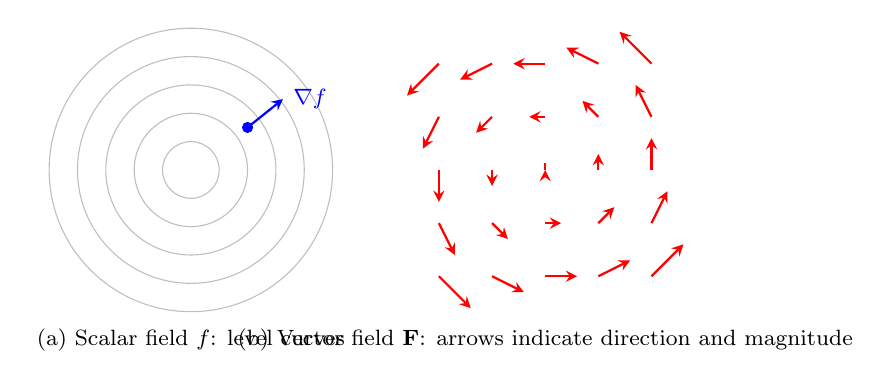
\begin{tikzpicture}[scale=0.9,>=stealth]
  % scalar field
  \begin{scope}[shift={(0,0)}]
    \foreach \r in {0.4,0.8,1.2,1.6,2.0}{
      \draw[gray!50] (0,0) circle (\r);
    }
    \node[font=\footnotesize] at (0,-2.4) {(a) Scalar field $f$: level curves};
    \filldraw[blue] (0.8,0.6) circle (2pt);
    \draw[->,thick,blue] (0.8,0.6) -- (1.3,1.0) node[right,font=\footnotesize]{$\nabla f$};
  \end{scope}
  % vector field
  \begin{scope}[shift={(5,0)}]
    \foreach \x in {-1.5,-0.75,0,0.75,1.5}{
      \foreach \y in {-1.5,-0.75,0,0.75,1.5}{
        \pgfmathsetmacro{\vx}{-\y}
        \pgfmathsetmacro{\vy}{\x}
        \draw[->,thick,red,>=stealth] (\x,\y) -- ({\x+0.3*\vx},{\y+0.3*\vy});
      }
    }
    \node[font=\footnotesize] at (0,-2.4) {(b) Vector field $\mathbf F$: arrows indicate direction and magnitude};
  \end{scope}
\end{tikzpicture}
\caption{Intuitive comparison of scalar and vector fields: a scalar field is represented by level curves, a vector field by arrows.}
\label{fig:scalar_vector_field}
\end{figure}

\begin{example}[The domain assumption is indispensable: a counterexample with a slit plane]\label{ex:slit_domain_counterexample}
Take $\mathcal{M} = \mathbb{R}^2 \setminus \{(x,0) : x \ge 0\}$ (the plane cut along the positive real axis); it is an open set but not simply connected. Consider
\[
\mathbf{F}(x,y) = \left( \frac{-y}{x^2+y^2},\; \frac{x}{x^2+y^2} \right).
\]
A direct computation gives $\nabla \times \mathbf{F} = \mathbf{0}$ everywhere on $\mathcal{M}$, but $\mathbf{F}$ has \textbf{no} scalar potential on $\mathcal{M}$: the circulation along a closed curve $\gamma$ winding once around the origin is $\oint_\gamma \mathbf F \cdot d\mathbf r = 2\pi \neq 0$.

\textbf{Conclusion}: $\nabla\times\mathbf F=\mathbf 0$ alone does not suffice to deduce the existence of a potential function; the simple connectivity of the domain must be added --- this is precisely why \cref{thm:irrotational_potential} has to write `$\mathcal{M}$ is simply connected' among its assumptions.
\end{example}

\begin{example}[Boundary regularity is indispensable: a counterexample with a needle-shaped region]\label{ex:needle_domain}
Take $\mathcal{M} = \{(x,y,z) : 0<x<1,\ 0<y<\varepsilon,\ 0<z<\varepsilon\}$ and keep at $x=1$ a contraction whose thickness tends to zero. As $\varepsilon \to 0$ a self-contacting sheet appears in $\partial\mathcal M$, and $\partial \mathcal M$ is then no longer a piecewise smooth closed surface.

\textbf{Conclusion}: the clause in the divergence theorem \cref{thm:divergence} that `$\partial V$ is a piecewise smooth closed surface and the outward normal $\mathbf n$ is well defined everywhere' cannot be omitted; on a needle-shaped limiting region the outward normal is not unique at the sheet, and the statement of the theorem itself fails (rather than its conclusion being false).
\end{example}

\section{The three basic transformations and the three differential operators}\label{sec:trans_scale_rotate}

This section is the hinge of the whole chapter. It answers two questions: why the three differential operators are `these three', and `what each of them corresponds to'.

\begin{remark}[The position of this section between the two sections]
This section places `transformations' and `operators' side by side in order to avoid a common confusion of expression: taking `the operator corresponding to translation is the gradient' as a definition, and then using the gradient in turn to `explain' translation. The order in this section is exactly the reverse --- first the three classes of transformations are defined independently and their group structure and range of generation are proved (\S\ref{subsec:trans_scale_rotate}), then the three operators are defined independently and their limit characterisations are proved (\S\ref{subsec:grad_div_curl}), and only then is the correspondence between the two discussed, with the exact meaning of that correspondence marked out level by level.
\end{remark}

\subsection{Translation, scaling and rotation}\label{subsec:trans_scale_rotate}

\begin{definition}[The translation transformation and the translation group]\label{def:translation_map}
Let $\mathbf{a} \in \mathbb{R}^n$. The map
\[
T_{\mathbf{a}}: \mathbb{R}^n \to \mathbb{R}^n, \qquad T_{\mathbf{a}}(\mathbf{x}) = \mathbf{x} + \mathbf{a}
\]
is called the \textbf{translation transformation} along the vector $\mathbf{a}$. Put
\[
\mathcal{T}_n = \{\, T_{\mathbf{a}} : \mathbf{a} \in \mathbb{R}^n \,\}.
\]

\textbf{Assumption}: $\mathbf a$ is a constant vector (independent of $\mathbf x$ and $t$); $n$ is arbitrary. The following \cref{lem:translation_group} shows that $\mathcal T_n$ forms a group under composition of maps.
\end{definition}

\begin{lemma}[The group structure of the translation group]\label{lem:translation_group}
$(\mathcal{T}_n, \circ)$ forms an Abelian group, and the map $\mathbf{a} \mapsto T_{\mathbf{a}}$ gives a group isomorphism
\[
(\mathcal{T}_n, \circ) \;\cong\; (\mathbb{R}^n, +).
\]
\end{lemma}

\begin{proof}
We verify the four group axioms and the isomorphism relation one by one.

\textbf{(1) Closure under composition}: for any $\mathbf{a}, \mathbf{b} \in \mathbb{R}^n$ and any $\mathbf{x} \in \mathbb{R}^n$,
\[
(T_{\mathbf{a}} \circ T_{\mathbf{b}})(\mathbf{x})
= T_{\mathbf{a}}\bigl(T_{\mathbf{b}}(\mathbf{x})\bigr)
= T_{\mathbf{a}}(\mathbf{x} + \mathbf{b})
= \mathbf{x} + \mathbf{b} + \mathbf{a}
= T_{\mathbf{a}+\mathbf{b}}(\mathbf{x}),
\]
hence $T_{\mathbf{a}} \circ T_{\mathbf{b}} = T_{\mathbf{a}+\mathbf{b}} \in \mathcal{T}_n$.

\textbf{(2) Associativity}: this follows directly from the associativity of composition,
$(T_{\mathbf a}\circ T_{\mathbf b})\circ T_{\mathbf c}=T_{\mathbf a}\circ(T_{\mathbf b}\circ T_{\mathbf c})$;
alternatively, by (1) both sides are computed to equal $T_{\mathbf a+\mathbf b+\mathbf c}$.

\textbf{(3) Identity element}: $T_{\mathbf{0}} = \mathrm{id}_{\mathbb R^n}$, and $T_{\mathbf a}\circ T_{\mathbf 0}=T_{\mathbf a}=T_{\mathbf 0}\circ T_{\mathbf a}$.

\textbf{(4) Inverse element}: by (1), $T_{\mathbf{a}} \circ T_{-\mathbf{a}} = T_{\mathbf{0}} = T_{-\mathbf{a}} \circ T_{\mathbf{a}}$, hence $(T_{\mathbf a})^{-1} = T_{-\mathbf a} \in \mathcal T_n$.

\textbf{(5) Isomorphism}: define $\Phi: \mathbb{R}^n \to \mathcal{T}_n$, $\Phi(\mathbf{a}) = T_{\mathbf{a}}$. By (1), $\Phi(\mathbf{a}+\mathbf{b}) = T_{\mathbf{a}+\mathbf{b}} = T_{\mathbf{a}} \circ T_{\mathbf{b}} = \Phi(\mathbf{a}) \circ \Phi(\mathbf{b})$, so $\Phi$ is a group homomorphism; $\Phi$ is surjective (as $T_{\mathbf a}=\Phi(\mathbf a)$ runs through $\mathcal T_n$); if $\Phi(\mathbf{a}) = \Phi(\mathbf{b})$, then $\mathbf x+\mathbf a=\mathbf x+\mathbf b$ for every $\mathbf x$, and taking $\mathbf x=\mathbf 0$ gives $\mathbf a=\mathbf b$, so $\Phi$ is injective. Thus $\Phi$ is an isomorphism, and an isomorphism carries the commutativity of the source group over to the image group.
\end{proof}

\begin{definition}[The scaling transformation and the scaling group]\label{def:scaling_map}
Let $\lambda \in \mathbb{R}_{>0}$. The map
\[
S_{\lambda}: \mathbb{R}^n \to \mathbb{R}^n, \qquad S_{\lambda}(\mathbf{x}) = \lambda \mathbf{x}
\]
is called the \textbf{(isotropic) scaling transformation}, and $\lambda$ is called the scaling factor. Put
\[
\mathcal{S}_n = \{\, S_{\lambda} : \lambda \in \mathbb{R}_{>0} \,\}.
\]

\textbf{Assumptions and boundary cases}: $\lambda > 0$ is essential. If $\lambda = 0$ were allowed, then $S_0$ would not be injective and $\mathcal S_n$ would no longer be a group; if $\lambda < 0$ were allowed, then $S_\lambda$ would contain a central inversion component and its composition relation with rotations would change. **Anisotropic** scaling $\mathrm{diag}(\lambda_1,\lambda_2,\lambda_3)$ (with the $\lambda_i$ not all equal) does not belong to $\mathcal S_n$; see \cref{ex:shear_anisotropic}.
\end{definition}

\begin{lemma}[The group structure of the scaling group]\label{lem:scaling_group}
$(\mathcal{S}_n, \circ)$ forms an Abelian group, and $\lambda \mapsto S_{\lambda}$ gives a group isomorphism
\[
(\mathcal{S}_n, \circ) \;\cong\; (\mathbb{R}_{>0}, \times).
\]
\end{lemma}

\begin{proof}
For $\mathbf{x}\in\mathbb R^n$, $(S_\lambda \circ S_\mu)(\mathbf{x}) = S_\lambda(\mu\mathbf{x}) = \lambda\mu\,\mathbf{x} = S_{\lambda\mu}(\mathbf{x})$, so the set is closed under composition and the operation is commutative. Associativity is given by the associativity of composition; the identity element is $S_1=\mathrm{id}$; the inverse element is $(S_\lambda)^{-1}=S_{1/\lambda}$ (since $\lambda>0$, $1/\lambda>0$ still lies in the index set). The isomorphism $\Psi(\lambda)=S_\lambda$ satisfies $\Psi(\lambda\mu)=\Psi(\lambda)\circ\Psi(\mu)$, and $\Psi$ is a bijection ($\lambda\mapsto S_\lambda$ and $S_\lambda\mapsto\lambda$ are mutually inverse).
\end{proof}

\begin{definition}[The rotation transformation and the rotation group]\label{def:rotation_map}
Let $\theta \in \mathbb{R}$. \textbf{Rotation about the origin} $R_\theta$ is given, when $n=2$, by the matrix
\[
R_\theta =
\begin{pmatrix}
\cos\theta & -\sin\theta \\
\sin\theta & \phantom{-}\cos\theta
\end{pmatrix},
\qquad
R_\theta(\mathbf{x}) = R_\theta\,\mathbf{x}.
\]
Put $\mathcal{R}_2 = \{R_\theta : \theta \in \mathbb{R}\}$. When $n=3$, the rotation about the unit axis $\mathbf{u}$ ($\|\mathbf{u}\|=1$) through the angle $\theta$ is written $R_{\mathbf{u},\theta}$, and its matrix is given by Rodrigues' formula
\[
R_{\mathbf{u},\theta}
= I + \sin\theta\,[\mathbf{u}]_\times + (1-\cos\theta)\,[\mathbf{u}]_\times^2,
\]
where $[\mathbf{u}]_\times \mathbf{v} = \mathbf{u}\times\mathbf{v}$.

\textbf{Assumption}: $R_\theta$ leaves the origin fixed; $\det R_\theta = 1$ ($\theta$ is a true rotation, containing no mirror); that $\mathbf u$ is a unit vector is the assumption under which Rodrigues' formula \textbf{contains no extra normalisation factor}.
\end{definition}

\begin{lemma}[The rotation group is isomorphic to the circle group]\label{lem:rotation_group}
$(a)$ When $n=2$, $(\mathcal{R}_2, \circ) \cong U(1) = \{z \in \mathbb{C} : |z| = 1\}$, and the isomorphism is given by $\theta \mapsto e^{i\theta}$, whose kernel is $2\pi\mathbb{Z}$.
$(b)$ When $n=3$, $(\mathcal{R}_3,\circ)\cong SO(3)$, and $SO(3) \cong SU(2)/\{\pm I\}$ (double cover).
\end{lemma}

\begin{proof}
$(a)$ A direct computation with matrix multiplication gives:
\[
R_\theta R_\varphi =
\begin{pmatrix}
\cos\theta\cos\varphi - \sin\theta\sin\varphi & -\cos\theta\sin\varphi - \sin\theta\cos\varphi \\
\sin\theta\cos\varphi + \cos\theta\sin\varphi & -\sin\theta\sin\varphi + \cos\theta\cos\varphi
\end{pmatrix}
= R_{\theta+\varphi},
\]
so $\theta \mapsto R_\theta$ is a surjective homomorphism from $(\mathbb R,+)$ onto $\mathcal R_2$. On the other hand, identifying $R_\theta$ with the complex number $e^{i\theta}=\cos\theta+i\sin\theta$ (the plane $\mathbb R^2 \cong \mathbb C$, $(x,y)\mapsto x+iy$), the action of $R_\theta$ is exactly multiplication by $e^{i\theta}$, so that $R_\theta R_\varphi = R_{\theta+\varphi}$ corresponds to $e^{i(\theta+\varphi)} = e^{i\theta}e^{i\varphi}$. Hence $\theta\mapsto e^{i\theta}$ is a surjective homomorphism whose kernel is $\{\theta : e^{i\theta}=1\} = 2\pi\mathbb Z$.

$(b)$ The first relation is a standard result of linear algebra (the set of all orthogonal matrices with determinant $1$ is precisely $SO(3)$). For the proof of the second, see the conjugation action $\rho_q$ given in \cref{thm:q_rotation}, where it is proved that $\rho: SU(2)\to SO(3)$ is a surjective homomorphism with $\ker\rho = \{\pm I\}$.
\end{proof}

\begin{proposition}[Fixed points and invariants of the three classes of transformations]\label{prop:transform_invariants}
Let $n=3$ and let the parameters be non-trivial ($\mathbf a \ne \mathbf 0$, $\lambda \ne 1$, $\theta \notin 2\pi\mathbb Z$). Then
\begin{enumerate}[label=(\roman*)]
    \item $T_{\mathbf a}$ has no fixed point; the geometric quantity it preserves is the difference $\mathbf x - \mathbf y$ of any two points (that is, it preserves displacement vectors and the distances between points), but it does not preserve the distance from a point to the origin.
    \item $S_\lambda$ has the unique fixed point $\mathbf{0}$; the geometric quantity it preserves is the family of lines through the origin (that is, directions), but it does not preserve distances between points (when $\lambda\ne1$).
    \item The fixed point set of $R_{\mathbf u,\theta}$ is the line $\mathbb R\mathbf u$; the geometric quantity it preserves is the inner product $\langle\mathbf x,\mathbf y\rangle$ (hence the norm and the angle), but it does not preserve direction (when $\theta\notin 2\pi\mathbb Z$).
\end{enumerate}
\end{proposition}

\begin{proof}
We verify the `fixed point equation' and the `invariants' item by item.

\textbf{(i)} The fixed point equation $\mathbf x = \mathbf x + \mathbf a$ is equivalent to $\mathbf a = \mathbf 0$, which contradicts $\mathbf a\ne\mathbf 0$; hence there is no fixed point. For any $\mathbf x,\mathbf y$, $T_{\mathbf a}(\mathbf x)-T_{\mathbf a}(\mathbf y)=(\mathbf x+\mathbf a)-(\mathbf y+\mathbf a)=\mathbf x-\mathbf y$, so both the difference vector and the distance between points $d(\mathbf x,\mathbf y)=\|\mathbf x-\mathbf y\|$ are preserved. Taking $\mathbf x=\mathbf 0$, $\|T_{\mathbf a}(\mathbf 0)\|=\|\mathbf a\|\ne 0=\|\mathbf 0\|$, so the distance to the origin is not preserved.

\textbf{(ii)} The fixed point equation $\mathbf x=\lambda\mathbf x$ is equivalent to $(\lambda-1)\mathbf x=\mathbf 0$, and since $\lambda\ne1$ we have $\mathbf x=\mathbf 0$ uniquely. For $\mu\in\mathbb R$ and $\mathbf x$, $S_\lambda(\mu\mathbf x)=\mu\lambda\mathbf x=\mu S_\lambda(\mathbf x)$, so $\mathbb R\mathbf x$ is mapped to itself and direction is preserved. As for distances, $\|S_\lambda(\mathbf x)-S_\lambda(\mathbf y)\|=\lambda\|\mathbf x-\mathbf y\|$, which is not equal when $\mathbf x\ne\mathbf y$ and $\lambda\ne1$.

\textbf{(iii)} The fixed point equation $R_{\mathbf u,\theta}\mathbf x=\mathbf x$. By Rodrigues' formula, for $\mathbf x=t\mathbf u$: $[\mathbf u]_\times\mathbf u=\mathbf u\times\mathbf u=\mathbf 0$, so $R_{\mathbf u,\theta}(t\mathbf u)=t\mathbf u$, that is, every point of $\mathbb R\mathbf u$ is fixed. Conversely, if $\mathbf x$ is fixed and $\mathbf x\notin\mathbb R\mathbf u$, then $\mathbf x$ and $\mathbf u$ span a two-dimensional plane, on which $R_{\mathbf u,\theta}$ restricts to a two-dimensional rotation through the angle $\theta\notin2\pi\mathbb Z$ (this is precisely the $\mathcal R_2$ case of \cref{lem:rotation_group}(a)), whose only fixed point is the origin --- a contradiction. Hence the fixed point set is exactly $\mathbb R\mathbf u$. Preservation of the inner product: $R_{\mathbf u,\theta}$ is an orthogonal matrix ($R^{\mathsf T}R=I$, $\det R=1$), and an orthogonal matrix preserves the standard inner product by definition, so $\langle R\mathbf x,R\mathbf y\rangle=\mathbf x^{\mathsf T}R^{\mathsf T}R\,\mathbf y=\langle\mathbf x,\mathbf y\rangle$. Non-preservation of direction: take $\mathbf x\perp\mathbf u$ with $\mathbf x\ne\mathbf 0$; then $R_{\mathbf u,\theta}\mathbf x\ne\mathbf x$ (otherwise $\mathbf x$ would be a fixed point with $\mathbf x\notin\mathbb R\mathbf u$, contradicting the preceding paragraph), so $\mathbb R\mathbf x\ne\mathbb R(R_{\mathbf u,\theta}\mathbf x)$.
\end{proof}

\begin{proposition}[The three symmetry centres]\label{prop:three_centres}
Each of the three classes of transformations leaves a \textbf{fixed structure}---a fixed point, or the cyclic subgroup generated by some element---on the group structure to which it belongs, and these three fixed structures are the three symmetry centres named by this programme:
\begin{enumerate}[label=(\roman*)]
    \item In the additive group $(\mathbb{R},+)$, the unique fixed point of the inversion $x \mapsto -x$ is $0$; correspondingly $T_{\mathbf a}$ degenerates to the identity when $\mathbf a=\mathbf 0$.
    \item In the multiplicative group $(\mathbb{R}_{>0},\times)$, the unique fixed point of the inversion $x \mapsto x^{-1}$ is $1$; correspondingly $S_\lambda$ degenerates to the identity when $\lambda=1$.
    \item In the circle group $U(1)$, the element $i = e^{i\pi/2}$ satisfies $i^4 = 1$ and $|i| = 1$; the cyclic subgroup $\{1,i,-1,-i\}=C_4$ that it generates is the fixed structure of the rotation case---$i$ is both a generator of $C_4$ and the multiplier corresponding to $R_{\pi/2}$; correspondingly $R_{\pi/2}$ corresponds to multiplication by $i$ when $n=2$.
\end{enumerate}
\end{proposition}

\begin{proof}
(i) From $-x=x$ we get $2x=0$, so $x=0$; uniqueness follows directly from that equation. (ii) From $x^{-1}=x$ and $x>0$ we get $x^2=1$, so $x=1$; uniqueness follows from the fact that for $x>0$ the equation $x^2=1$ has the positive solution $1$ only. (iii) $i=e^{i\pi/2}=\cos\frac\pi2+i\sin\frac\pi2$, so $|i|=1$ and $i^4=e^{i2\pi}=1$; moreover $\{i^k:k=0,1,2,3\}=\{1,i,-1,-i\}$ is the cyclic subgroup of $U(1)$ generated by $i$. When $n=2$ the matrix of $R_{\pi/2}$ is $\left(\begin{smallmatrix}0&-1\\1&0\end{smallmatrix}\right)$, whilst multiplication by $i$ in real coordinates is exactly $(x,y)\mapsto(-y,x)$; the two agree.
\end{proof}

\begin{remark}[How the three symmetry centres are related to the two groups of objects]\label{rem:centres_and_two_triples}
The three symmetry centres $0$, $1$, $i$ are the common pivot of the whole book, and each of them is associated both with a basic transformation and with a differential operator:
\[
0 \;\longleftrightarrow\; \text{translation},\quad \nabla f;
\qquad
1 \;\longleftrightarrow\; \text{scaling},\quad \nabla\cdot\mathbf{F};
\qquad
i \;\longleftrightarrow\; \text{rotation},\quad \nabla\times\mathbf{F}.
\]
\textbf{What is recorded here is the association between each symmetry centre $\leftrightarrow$ its respective object, not a correspondence between the two groups of objects.} The two groups of objects lie at different levels --- transformations act on space, operators act on fields (scalar fields and vector fields) --- and arranging them in a table of mutual correspondence would obscure the true assumptions under which each holds. The principle of this book is therefore: wherever translation, scaling or rotation is involved, state matters according to the assumptions of the transformation itself; wherever gradient, divergence or curl is involved, state matters according to the differentiability and domain assumptions of the operator itself; and make no assertion of correspondence between the two groups.
\end{remark}

\begin{proposition}[The range generated by the three is exactly the orientation-preserving similitude group]\label{prop:similitude_group}
Let $\mathrm{Sim}^{+}(n)$ denote the \textbf{orientation-preserving similitude transformation group} of Euclidean space $\mathbb R^n$, that is, the set of all maps of the form
\[
\mathbf x \mapsto \lambda R\,\mathbf x + \mathbf a, \qquad \lambda>0,\ R\in SO(n),\ \mathbf a\in\mathbb R^n .
\]
Then the group generated by translation, scaling and rotation is equal to $\mathrm{Sim}^{+}(n)$:
\[
\langle \mathcal{T}_n,\ \mathcal{S}_n,\ \mathcal{R}_n\rangle = \mathrm{Sim}^{+}(n).
\]
Consequently, no continuous transformation outside $\mathrm{Sim}^{+}(n)$ can be expressed as a finite composite of these three classes of transformations.

\textbf{Boundary remark}: the group in this conclusion is $\mathrm{Sim}^{+}(n)$ and not the full similitude group $\mathrm{Sim}(n)=\mathbb R^n\rtimes(\mathbb R_{>0}\times O(n))$, which contains reflections. A reflection matrix has determinant $-1$, whilst the linear part of every element of $\mathcal T_n,\mathcal S_n,\mathcal R_n$ has positive determinant, so a reflection \textbf{cannot} be obtained as a composite of the three; see \cref{rem:transform_group_relations}.
\end{proposition}

\begin{proof}
\textbf{(1) The inclusion $\subseteq$}: every element of $\mathcal T_n$, $\mathcal S_n$, $\mathcal R_n$ has the form $\mathbf x\mapsto\lambda R\mathbf x+\mathbf a$, and the determinant of $R$ is $1$ (translation takes $\lambda=1,R=I$; scaling takes $R=I,\mathbf a=\mathbf 0$; rotation takes $\lambda=1,\mathbf a=\mathbf 0$, and by \cref{def:rotation_map} $\det R_{\mathbf u,\theta}=1$). Maps of this kind are closed under composition: if $g_i(\mathbf x)=\lambda_iR_i\mathbf x+\mathbf a_i$ ($i=1,2$), then
\[
g_1(g_2(\mathbf x)) = \lambda_1R_1(\lambda_2R_2\mathbf x+\mathbf a_2)+\mathbf a_1
= (\lambda_1\lambda_2)(R_1R_2)\mathbf x + (\lambda_1R_1\mathbf a_2+\mathbf a_1),
\]
where $\lambda_1\lambda_2>0$, $\det(R_1R_2)=\det R_1\det R_2=1$ and $\lambda_1R_1\mathbf a_2+\mathbf a_1\in\mathbb R^n$, so the composite still lies in $\mathrm{Sim}^{+}(n)$. Hence every finite composite lies in $\mathrm{Sim}^{+}(n)$.

\textbf{(2) The inclusion $\supseteq$}: let $g(\mathbf x)=\lambda R\mathbf x+\mathbf a$ be any orientation-preserving similitude transformation, where $R\in SO(n)$. By linear algebra: when $n=2$, $SO(2)=\mathcal R_2$, so $R\in\langle\mathcal R_2\rangle$; when $n=3$, every $R\in SO(3)$ is a rotation about some unit axis $\mathbf u$ through an angle $\theta$ (Euler's theorem), that is, $R=R_{\mathbf u,\theta}\in\mathcal R_3$. Hence $R\in\langle\mathcal R_n\rangle$. Also
\[
g = T_{\mathbf a}\circ S_\lambda\circ R,
\]
because for any $\mathbf x$: $R(\mathbf x)=R\mathbf x$, $S_\lambda(R\mathbf x)=\lambda R\mathbf x$, $T_{\mathbf a}(\lambda R\mathbf x)=\lambda R\mathbf x+\mathbf a=g(\mathbf x)$. Hence $g\in\langle\mathcal T_n,\mathcal S_n,\mathcal R_n\rangle$.
\end{proof}

\begin{example}[Counterexample: the shear transformation and anisotropic scaling do not belong to the similitude group]\label{ex:shear_anisotropic}
Take the shear matrix $A_t = \left(\begin{smallmatrix}1 & t\\ 0 & 1\end{smallmatrix}\right)$ ($t\ne0$); it preserves area ($|\det A_t|=1$) and orientation, and is a smooth continuous transformation. Take the anisotropic scaling $B=\mathrm{diag}(2,1)$; it is smooth as well.

\textbf{Argument that neither belongs to $\mathrm{Sim}(2)$}: the matrix of the linear part of an element of $\mathrm{Sim}(2)$ must be $\lambda R_\theta$, satisfying $(M^{\mathsf T}M)^{1/2}=\lambda I$, that is, $M^{\mathsf T}M$ is a scalar matrix. But
\[
A_t^{\mathsf T}A_t=\begin{pmatrix}1&t\\ t&1+t^2\end{pmatrix},\qquad
B^{\mathsf T}B=\begin{pmatrix}4&0\\0&1\end{pmatrix},
\]
and in both cases $M^{\mathsf T}M$ fails to be a scalar matrix (for the former, the off-diagonal entry is non-zero when $t\ne0$; for the latter, the diagonal entries are unequal). Hence $A_t,B\notin\mathrm{Sim}^{+}(2)$, and by \cref{prop:similitude_group} neither can be written as a finite composite of translations, scalings and rotations.

\textbf{Significance}: this gives concrete evidence for the statement in \cref{rem:transform_scope} that `the three are not all continuous transformations': there exist smooth transformations preserving some intrinsic structure (preserving area, or preserving a certain coordinate direction) that do not fall into the group generated by the three.
\end{example}

\begin{remark}[The scope of validity of the three classes of transformations]\label{rem:transform_scope}
This section establishes translation, scaling and rotation as \textbf{candidate} generators, on the basis of motivations at three levels (algebra: the three correspond respectively to the additive group, the multiplicative group and the circle group; geometry: the three exactly exhaust the continuous transformations of similarity geometry that do not change the intrinsic structure; number systems: subtraction, division and complex roots introduce respectively the directions of translation, proportion and rotation), and not on the basis of the following proposition:

\begin{center}
\textit{`Any continuous transformation preserving some intrinsic structure can be decomposed into a composite of elements of these three groups.'}
\end{center}

\textbf{That proposition is a research programme, not a proved theorem.} By \cref{prop:similitude_group} and \cref{ex:shear_anisotropic} we know: if `intrinsic structure' is understood as \textbf{Euclidean similarity structure}, then the proposition holds (in which case it is precisely \cref{prop:similitude_group}); if `intrinsic structure' is relaxed to area, volume, parallelism in some direction, or any other invariant, then the proposition is \textbf{false}. Hence wherever this book uses the proposition it must specify the intrinsic structure taken, and any use without such a specification is treated as a research programme.
\end{remark}

\begin{example}[Three standard examples of the three classes of transformations]
(i) \textbf{Translation}: on a train moving at constant speed, each time the wheels rotate once a mark on the carriage floor returns to the same position --- the displacement vector is preserved throughout. (ii) \textbf{Scaling}: the boundary of the Koch snowflake returns to itself under each scaling transformation by $\times 3$ (the boundary curve after magnification by $3$ has the same structure as before magnification), its perimeter is infinite whilst its area is finite, and it is the area that is precisely the invariant making the scaling `closed'. (iii) \textbf{Rotation}: the revolution of the Earth around the Sun is, in the approximation that neglects the perturbations of the other planets, a closed orbit in a rotationally symmetric system, and its angular momentum is conserved.
\end{example}

\begin{figure}[htbp]
    \centering
    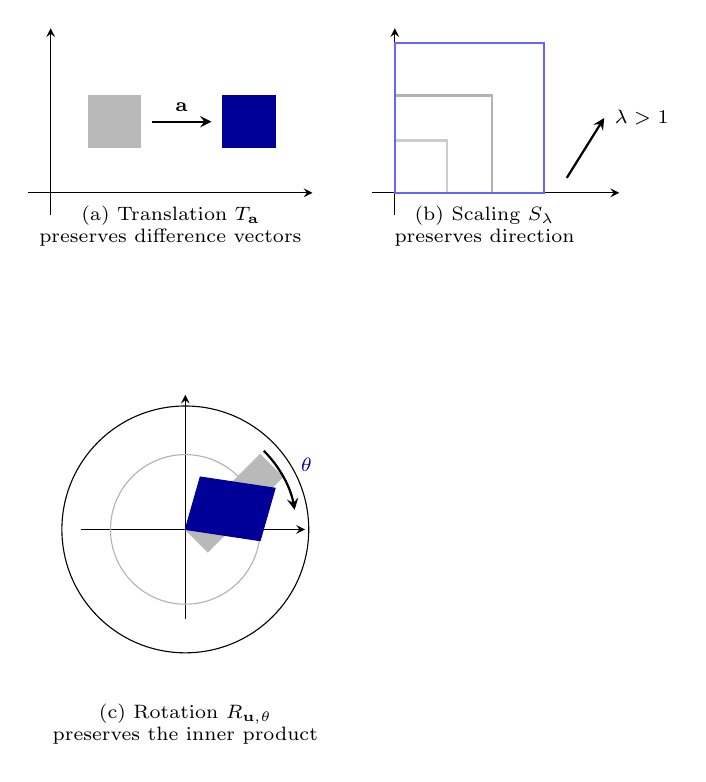
\begin{tikzpicture}[scale=0.95,>=stealth]

        \begin{scope}[shift={(0,0)}]
            \draw[->] (-0.3,0) -- (3.5,0);
            \draw[->] (0,-0.3) -- (0,2.2);
            \filldraw[gray!55] (0.5,0.6) -- (1.2,0.6) -- (1.2,1.3) -- (0.5,1.3) -- cycle;
            \draw[gray!55,dashed] (0.5,0.6) -- (1.2,0.6) -- (1.2,1.3);
            \draw[->,thick] (1.35,0.95) -- (2.15,0.95) node[midway,above,font=\scriptsize]{$\mathbf a$};
            \filldraw[blue!60!black] (2.3,0.6) -- (3.0,0.6) -- (3.0,1.3) -- (2.3,1.3) -- cycle;
            \node[font=\scriptsize,align=center] at (1.6,-0.45) {(a) Translation $T_{\mathbf a}$\\preserves difference vectors};
        \end{scope}

        \begin{scope}[shift={(4.6,0)}]
            \draw[->] (-0.3,0) -- (3.0,0);
            \draw[->] (0,-0.3) -- (0,2.2);

            \draw[thick,gray!40] (0,0) rectangle (0.7,0.7);
            \draw[thick,gray!60] (0,0) rectangle (1.3,1.3);
            \draw[thick,blue!60] (0,0) rectangle (2.0,2.0);
            \draw[->,thick] (2.3,0.2) -- (2.8,1.0) node[right,font=\scriptsize]{$\lambda>1$};
            \node[font=\scriptsize,align=center] at (1.2,-0.45) {(b) Scaling $S_\lambda$\\preserves direction};
        \end{scope}
\begin{scope}[shift={(1.8,-4.5)}]
            \draw[->] (-1.4,0) -- (1.6,0);
            \draw[->] (0,-1.2) -- (0,1.8);
            \draw[gray!60] (0,0) circle (1.0);
            \filldraw[gray!55] (0,0) -- (1.0,1.0) -- (1.3,0.7) -- (0.3,-0.3) -- cycle;
            \draw[->,thick] (1.05,1.05) arc (45:10:1.48);
            \node[blue!60!black,font=\scriptsize] at (1.62,0.86) {$\theta$};
            \filldraw[blue!60!black] (0,0) -- (1.0,-0.15) -- (1.2,0.55) -- (0.2,0.7) -- cycle;
            \draw[thin] (0,0) circle (1.65);

            \node[font=\scriptsize,align=center,yshift=-1cm] at (0,-1.55) {(c) Rotation $R_{\mathbf u,\theta}$\\preserves the inner product};
        \end{scope}
    \end{tikzpicture}
    \caption{The three basic transformations and their invariants. Each of the three classes of transformations preserves a different geometric quantity: translation preserves the difference vector between points, scaling preserves directions through the origin, and rotation preserves the inner product; \cref{prop:transform_invariants} gives the proof of each item.}
    \label{fig:three_basic_transforms}
\end{figure}

\begin{table}[htbp]
    \centering
    \caption{Structural comparison of the three basic transformations}
    \label{tab:transform_summary}
    \renewcommand{\arraystretch}{1.35}
    \begin{tabularx}{\textwidth}{@{}l l l l X@{}}
        \toprule
        \textbf{Transformation} & \textbf{Group} & \textbf{Isomorphic to} & \textbf{Fixed point set} & \textbf{Geometric quantity preserved} \\
        \midrule
        Translation $T_{\mathbf a}$ & $\mathcal T_n$ & $(\mathbb R^n,+)$ & empty ($\mathbf a\ne\mathbf 0$) & difference vector $\mathbf x-\mathbf y$, distance between points \\
        Scaling $S_\lambda$ & $\mathcal S_n$ & $(\mathbb R_{>0},\times)$ & $\{\mathbf 0\}$ ($\lambda\ne1$) & directions through the origin $\mathbb R\mathbf x$ \\
        Rotation $R_{\mathbf u,\theta}$ & $\mathcal R_n$ & $U(1)$ ($n=2$) & $\mathbb R\mathbf u$ ($n=3$) & inner product $\langle\mathbf x,\mathbf y\rangle$, norm, angle \\
        \bottomrule
    \end{tabularx}
\end{table}

\begin{remark}[The group-representation-theoretic relations among the three]\label{rem:transform_group_relations}
By \cref{lem:translation_group}--\cref{lem:rotation_group}, both $\mathcal T_n$ and $\mathcal S_n$ are Abelian groups, whilst $\mathcal R_n$ is non-Abelian when $n=3$. The interaction of the three is not a direct product but a semidirect product: the translation subgroup $\mathcal T_n$ is a normal subgroup of $\mathrm{Sim}^{+}(n)$, and
\[
\mathrm{Sim}^{+}(n) = \mathcal T_n \rtimes \bigl(\mathcal S_n \times SO(n)\bigr),
\]
where $\mathcal S_n\times SO(n)$ acts on $\mathcal T_n$ by $(\lambda,R)\cdot\mathbf a \mapsto \lambda R\mathbf a$. This semidirect product structure explains the phenomenon that `scale first and then translate' and `translate first and then scale' give different results: the action is not translation invariant.

\textbf{Boundary warning}: the full similitude group also contains reflections, $\mathrm{Sim}(n)=\mathcal T_n\rtimes(\mathcal S_n\times O(n))\supsetneq\mathrm{Sim}^{+}(n)$; the linear part of a reflection has determinant $-1$, whilst the linear parts of $\mathcal T_n,\mathcal S_n,\mathcal R_n$ all have determinant $1$, so a reflection does not belong to the group generated by the three (see the boundary remark of \cref{prop:similitude_group}). The remainder of this chapter uses only the orientation-preserving similitude group.
\end{remark}

\subsection{Gradient, divergence and curl}\label{subsec:grad_div_curl}

The preceding subsection gave the three classes of transformations; this subsection gives the three differential operators and explains \textbf{exactly how far} their relation to the three classes of transformations goes. The order here is deliberate: the three operators are first defined independently by coordinate formulae (\cref{def:nabla}--\cref{def:curl_vf}), then reduced by two limit characterisations to geometric quantities independent of the coordinate system (\cref{prop:divergence_flux_density} and \cref{prop:curl_circulation_density}), and only then is their status as infinitesimal generators of the three classes of transformations discussed (\cref{thm:infinitesimal_generators}).

\begin{definition}[The nabla operator]\label{def:nabla}
In $\mathbb{R}^3$, define the formal vector operator $\nabla$ (read as nabla or del) by
\[
\nabla = \left( \frac{\partial}{\partial x},\; \frac{\partial}{\partial y},\; \frac{\partial}{\partial z} \right).
\]

\textbf{Assumptions, and a fashionable phrasing distinguished}: $\nabla$ itself is \textbf{not} a vector in $\mathbb R^3$ --- it belongs to no tangent space and has neither length nor direction; it is a \textbf{vector-valued differential operator}, that is, a triple `each of whose components is a partial derivative operator acting on $C^1$ functions'. Writing it as a triple is merely a notational convenience: $\nabla f$ is defined because $\partial/\partial x$ acts on $f$, not because `$\nabla$ is multiplied by $f$'.

\textbf{Well-definedness}: $\nabla$ acts on fields in three ways, and each action requires the object acted upon to possess continuous differentiability of the corresponding order (see \cref{def:gradient_vf}--\cref{def:curl_vf}); when that order is not satisfied, the corresponding action of $\nabla$ is \textbf{undefined}, rather than `having the value zero'.
\end{definition}

\begin{definition}[Gradient]\label{def:gradient_vf}
The first definition of the gradient operator is to be found in chapter~\ref{chap:diffeq_complex}, \cref{sec:grad_curl_div}, in \cref{def:gradient}; this section presents the same object in the framework of $C^1$ open sets and supplements the differentiability assumptions and the mapping type.
Let $f \in C^1(\mathcal{M})$ be a scalar field ($\mathcal M\subseteq\mathbb R^3$ a non-empty open set). The \textbf{gradient} of $f$ is a vector field $\nabla f: \mathcal{M} \to \mathbb{R}^3$, defined by
\[
\nabla f(x,y,z) = \left( \frac{\partial f}{\partial x}(x,y,z),\; \frac{\partial f}{\partial y}(x,y,z),\; \frac{\partial f}{\partial z}(x,y,z) \right).
\]

\textbf{Assumption}: $f\in C^1$ is a sufficient condition; if $f$ is differentiable only at a single point, then $\nabla f$ is defined only at that point. The mapping type is
\[
\nabla: C^1(\mathcal{M}) \to C^0(\mathcal{M}, \mathbb{R}^3),
\]
that is, the gradient \textbf{raises the order} (a scalar field becomes a vector field). It is linear, but it does not preserve multiplication (see \cref{thm:product_rules}(i)).
\end{definition}

\begin{definition}[Divergence]\label{def:divergence_vf}
The first definition of the divergence operator is to be found in chapter~\ref{chap:diffeq_complex}, \cref{sec:grad_curl_div}, in \cref{def:divergence}; this section presents the same object in the framework of $C^1$ open sets and supplements the differentiability assumptions and the mapping type.
Let $\mathbf{F} = (F_1, F_2, F_3) \in C^1(\mathcal{M}, \mathbb{R}^3)$ be a vector field. The \textbf{divergence} of $\mathbf{F}$ is a scalar field $\nabla \cdot \mathbf{F}: \mathcal{M} \to \mathbb{R}$, defined by
\[
\nabla \cdot \mathbf{F}(x,y,z) = \frac{\partial F_1}{\partial x} + \frac{\partial F_2}{\partial y} + \frac{\partial F_3}{\partial z}.
\]

\textbf{Assumption}: $\mathbf F\in C^1$. The mapping type is
\[
\nabla\cdot: C^1(\mathcal{M}, \mathbb{R}^3) \to C^0(\mathcal{M}).
\]
\textbf{Note}: the defining formula of the divergence depends on the coordinate system, but its value does not depend on the choice of coordinate system (the limit characterisation given by \cref{prop:divergence_flux_density} is independent of this); this point, which is the same as for the curl, is a key repeatedly used in this chapter.
\end{definition}

\begin{definition}[Curl]\label{def:curl_vf}
The first definition of the curl operator is to be found in chapter~\ref{chap:diffeq_complex}, \cref{sec:grad_curl_div}, in \cref{def:curl}; this section presents the same object in the framework of $C^1$ open sets and supplements the differentiability assumptions and the mapping type.
Let $\mathbf{F} = (F_1, F_2, F_3) \in C^1(\mathcal{M}, \mathbb{R}^3)$ be a vector field. The \textbf{curl} of $\mathbf{F}$ is a vector field $\nabla \times \mathbf{F}: \mathcal{M} \to \mathbb{R}^3$, defined by the formal cross product
\[
\nabla \times \mathbf{F} = \begin{vmatrix}
\mathbf{i} & \mathbf{j} & \mathbf{k} \\[2pt]
\dfrac{\partial}{\partial x} & \dfrac{\partial}{\partial y} & \dfrac{\partial}{\partial z} \\[6pt]
F_1 & F_2 & F_3
\end{vmatrix}
= \left( \frac{\partial F_3}{\partial y} - \frac{\partial F_2}{\partial z},\;
\frac{\partial F_1}{\partial z} - \frac{\partial F_3}{\partial x},\;
\frac{\partial F_2}{\partial x} - \frac{\partial F_1}{\partial y} \right).
\]

\textbf{Assumption}: $\mathbf F\in C^1$. The determinant notation is merely a formal notation: treating a differential operator as a row of a determinant and expanding along the first row gives the formula above, but one \textbf{cannot} conclude from this that $\nabla$ and $\mathbf F$ commute --- in fact $\nabla\times\mathbf F$ and $\mathbf F\times\nabla$ differ by a sign (see \cref{prop:product_rules_orientation}). The mapping type is
\[
\nabla\times: C^1(\mathcal{M}, \mathbb{R}^3) \to C^0(\mathcal{M}, \mathbb{R}^3).
\]
\end{definition}

\begin{definition}[The Laplacian]\label{def:laplacian}
Let $f \in C^2(\mathcal{M})$ be a scalar field. The \textbf{Laplacian} of $f$ is a scalar field $\nabla^2 f: \mathcal{M} \to \mathbb{R}$, defined as the divergence of the gradient:
\[
\nabla^2 f = \nabla \cdot (\nabla f) = \frac{\partial^2 f}{\partial x^2} + \frac{\partial^2 f}{\partial y^2} + \frac{\partial^2 f}{\partial z^2}.
\]
For a vector field $\mathbf{F} = (F_1, F_2, F_3) \in C^2(\mathcal{M}, \mathbb{R}^3)$, its Laplacian is defined componentwise: $\nabla^2 \mathbf{F} = (\nabla^2 F_1,\; \nabla^2 F_2,\; \nabla^2 F_3)$.

\textbf{Assumption}: the scalar case requires $f\in C^2$; the vector case requires $\mathbf F\in C^2(\mathcal M,\mathbb R^3)$. If $f$ lies only in $C^1$, then $\nabla^2 f$ need not exist --- $\nabla f$ lies only in $C^0$, and taking its divergence again requires $C^1$, so $C^2$ is the minimum requirement.

If $\nabla^2 f = 0$ holds on $\mathcal{M}$, then $f$ is called a \textbf{harmonic function}.
\end{definition}

\begin{figure}[htbp]
\centering
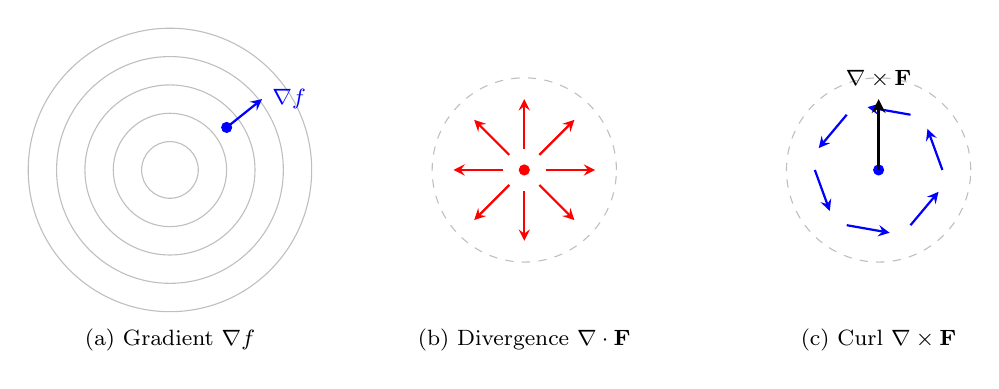
\begin{tikzpicture}[scale=0.9,>=stealth]
  % gradient
  \begin{scope}[shift={(0,0)}]
    \foreach \r in {0.4,0.8,1.2,1.6,2.0}{
      \draw[gray!50] (0,0) circle (\r);
    }
    \node[font=\footnotesize] at (0,-2.4) {(a) Gradient $\nabla f$};
    \filldraw[blue] (0.8,0.6) circle (2pt);
    \draw[->,thick,blue] (0.8,0.6) -- (1.3,1.0) node[right,font=\footnotesize]{$\nabla f$};
  \end{scope}
  % divergence
  \begin{scope}[shift={(5,0)}]
    \filldraw[red] (0,0) circle (2pt);
    \foreach \a in {0,45,...,315}{
      \draw[->,thick,red] (\a:0.3) -- (\a:1.0);
    }
    \draw[gray!50,dashed] (0,0) circle (1.3);
    \node[font=\footnotesize] at (0,-2.4) {(b) Divergence $\nabla\cdot\mathbf F$};
  \end{scope}
  % curl
  \begin{scope}[shift={(10,0)}]
    \foreach \a in {0,60,...,300}{
      \draw[->,thick,blue] (\a:0.9) -- ({\a+40}:0.9);
    }
    \draw[gray!50,dashed] (0,0) circle (1.3);
    \filldraw[blue] (0,0) circle (2pt);
    \draw[->,very thick] (0,0) -- (0,1.0) node[above,font=\footnotesize]{$\nabla\times\mathbf F$};
    \node[font=\footnotesize] at (0,-2.4) {(c) Curl $\nabla\times\mathbf F$};
  \end{scope}
\end{tikzpicture}
\caption{The geometric picture of the three differential operators: the gradient points in the direction of fastest increase, the divergence describes sources and sinks, and the curl describes local circulation.}
\label{fig:operators_geometry}
\end{figure}

\begin{lemma}[Two fundamental integral identities on a sphere]\label{lem:sphere_flux_identities}
Let $B_r = B_r(\mathbf{x}_0)$ be the closed ball in $\mathbb R^3$ with centre $\mathbf x_0$ and radius $r>0$, let $\partial B_r$ be its boundary sphere, $\mathbf n$ the unit outward normal, $dS$ the area element, and $|B_r| = \tfrac43\pi r^3$. Then
\begin{enumerate}[label=(\roman*)]
    \item $\displaystyle \oint_{\partial B_r} \mathbf{n} \, dS = \mathbf{0}$;
    \item $\displaystyle \oint_{\partial B_r} (\mathbf{x}-\mathbf{x}_0)_i\, n_j \, dS = |B_r| \, \delta_{ij}$, where $(\mathbf{x}-\mathbf{x}_0)_i$ and $n_j$ denote the $i$-th and $j$-th coordinate components respectively.
\end{enumerate}
\end{lemma}

\begin{proof}
Write $\mathbf y = \mathbf x-\mathbf x_0$, $\hat{\mathbf y} = \mathbf y/|\mathbf y|$. On $\partial B_r$ we have $|\mathbf y| = r$ and $\mathbf n = \hat{\mathbf y}$, whilst the area element of a sphere centred at $\mathbf x_0$ satisfies $dS = r^2\,d\Omega$, where $d\Omega$ is the area element on the unit sphere $S^2$ (this relation comes from the Jacobian factor $r^2$ of the spherical parametrisation $(r,\theta,\varphi)\mapsto \mathbf x_0+r\,\hat{\mathbf y}(\theta,\varphi)$).

\textbf{(i)} On the unit sphere $\oint_{S^2} \hat y_i \, d\Omega = 0$: the map $\hat{\mathbf y}\mapsto -\hat{\mathbf y}$ is a diffeomorphism of $S^2$ preserving the area element $d\Omega$ (since it is an orthogonal transformation with Jacobian factor $1$), but it carries $\hat y_i$ to $-\hat y_i$. Hence the integral equals its own negative, and can only be $0$. Therefore
$\oint_{\partial B_r}\mathbf n\,dS = \oint_{S^2} \hat{\mathbf y}\,r^2d\Omega = r^2\oint_{S^2}\hat{\mathbf y}\,d\Omega=\mathbf 0$.

\textbf{(ii)} First compute the integral over the unit sphere, $I_{ij} = \oint_{S^2}\hat y_i\hat y_j\,d\Omega$.

\emph{The off-diagonal case $i\ne j$}: let $i\ne j$ and consider the reflection $R_j: \hat{\mathbf y}\mapsto \hat{\mathbf y}'$ in the coordinate hyperplane $y_j = 0$, where $\hat y_j' = -\hat y_j$ and the other components are unchanged. $R_j$ is an orthogonal transformation, hence preserves $d\Omega$; it leaves $\hat y_i$ unchanged and changes the sign of $\hat y_j$, so the integrand $\hat y_i\hat y_j$ changes sign. Hence $I_{ij} = -I_{ij}$, giving $I_{ij}=0$.

\emph{The diagonal case}: by the symmetry above, the three diagonal entries are equal: $I_{11}=I_{22}=I_{33}$ (a permutation of coordinates is an orthogonal transformation preserving $d\Omega$ and permuting the diagonal integrals); whilst on $\hat y_1^2+\hat y_2^2+\hat y_3^2 = 1$,
\[
I_{11}+I_{22}+I_{33} = \oint_{S^2} (\hat y_1^2+\hat y_2^2+\hat y_3^2)\,d\Omega = \oint_{S^2} 1\,d\Omega = 4\pi .
\]
Hence each diagonal entry equals $\tfrac{4\pi}{3}$, that is, $I_{ij} = \tfrac{4\pi}{3}\delta_{ij}$.

Returning to the sphere: $\mathbf x-\mathbf x_0 = r\hat{\mathbf y}$ and $\mathbf n = \hat{\mathbf y}$, so
\[
\oint_{\partial B_r}(\mathbf x-\mathbf x_0)_i\,n_j\,dS
= \oint_{S^2} r\hat y_i\,\hat y_j\; r^2 d\Omega
= r^3 I_{ij}
= r^3\cdot\frac{4\pi}{3}\delta_{ij}
= \frac{4}{3}\pi r^3\,\delta_{ij}
= |B_r|\,\delta_{ij}. \qedhere
\]
\end{proof}

\begin{proposition}[The gradient and directional derivatives]\label{prop:gradient_directional}
Let $f \in C^1(\mathcal{M})$, $\mathbf{x}_0 \in \mathcal{M}$, and let $\mathbf{u}$ be a unit vector. Then
\[
D_{\mathbf{u}} f(\mathbf{x}_0) := \lim_{h\to0}\frac{f(\mathbf{x}_0+h\mathbf{u})-f(\mathbf{x}_0)}{h} = \nabla f(\mathbf{x}_0)\cdot\mathbf{u}.
\]
\end{proposition}

\begin{proof}
Since $f\in C^1(\mathcal M)$ and $f$ is defined in some neighbourhood of $\mathbf x_0$, $f$ is differentiable at $\mathbf x_0$ (the existence of continuous partial derivatives implies differentiability), that is, there is a linear map $L = Df(\mathbf x_0)$ such that
\[
f(\mathbf x_0+\mathbf h) = f(\mathbf x_0) + L\mathbf h + o(\|\mathbf h\|)\qquad(\|\mathbf h\|\to0).
\]
Here $L\mathbf h = \sum_i \partial_i f(\mathbf x_0)\,h_i = \nabla f(\mathbf x_0)\cdot\mathbf h$ (because the $i$-th component of $L$ is the directional derivative $\partial_i f$ along $e_i$, and $\{e_i\}$ is an orthogonal basis, so the pairing of $L\mathbf h$ with $\mathbf h$ is given by the standard inner product). Take $\mathbf h = h\mathbf u$ and divide by $h$ ($h\ne0$):
\[
\frac{f(\mathbf x_0+h\mathbf u)-f(\mathbf x_0)}{h}
= \frac{h\,\nabla f(\mathbf x_0)\cdot\mathbf u + o(|h|)}{h}
= \nabla f(\mathbf x_0)\cdot\mathbf u + \frac{o(|h|)}{h}.
\]
Since $o(|h|)/h \to 0$ as $h\to0$, taking the limit gives the conclusion.
\end{proof}

\begin{proposition}[The divergence is the flux density]\label{prop:divergence_flux_density}
Let $\mathbf{F} \in C^1(\mathcal{M}, \mathbb{R}^3)$, $\mathbf{x}_0 \in \mathcal{M}$, and $B_r = B_r(\mathbf{x}_0) \subseteq \mathcal M$ (with $r$ sufficiently small). Then
\[
\nabla \cdot \mathbf{F}(\mathbf{x}_0)
= \lim_{r \to 0^{+}} \frac{1}{|B_r|}\oint_{\partial B_r} \mathbf{F} \cdot \mathbf{n} \, dS .
\]
Equivalently, $(\nabla\cdot\mathbf F)(\mathbf x_0)$ is the \textbf{flux density} of $\mathbf F$ at $\mathbf x_0$ --- the net outward flux per unit volume.
\end{proposition}

\begin{proof}
Fix $\mathbf{x}_0$ and write $J = D\mathbf F(\mathbf x_0)$ (a $3\times3$ matrix, $J_{ij} = \partial_j F_i(\mathbf x_0)$). Since $\mathbf F$ is differentiable at $\mathbf x_0$, expand $\mathbf F$ to first order:
\[
\mathbf F(\mathbf x) = \mathbf F(\mathbf x_0) + J(\mathbf x-\mathbf x_0) + \mathbf R(\mathbf x),
\qquad \mathbf R(\mathbf x) = o(\|\mathbf x-\mathbf x_0\|)\;(\mathbf x\to\mathbf x_0).
\]
Split the flux into three parts:
\[
\oint_{\partial B_r}\mathbf F\cdot\mathbf n\,dS
= \underbrace{\mathbf F(\mathbf x_0)\cdot\oint_{\partial B_r}\mathbf n\,dS}_{T_1}
+ \underbrace{\oint_{\partial B_r} J(\mathbf x-\mathbf x_0)\cdot\mathbf n\,dS}_{T_2}
+ \underbrace{\oint_{\partial B_r}\mathbf R\cdot\mathbf n\,dS}_{T_3}.
\]

\textbf{$T_1$}: by \cref{lem:sphere_flux_identities}(i), $\oint \mathbf n\,dS = \mathbf 0$, so $T_1=0$.

\textbf{$T_2$}: write $J(\mathbf x-\mathbf x_0)\cdot\mathbf n = \sum_{i,j} J_{ij}(\mathbf x-\mathbf x_0)_j n_i$, integrate term by term and use \cref{lem:sphere_flux_identities}(ii):
\[
T_2 = \sum_{i,j} J_{ij}\oint_{\partial B_r}(\mathbf x-\mathbf x_0)_j n_i\,dS
= \sum_{i,j} J_{ij}\,|B_r|\,\delta_{ij}
= |B_r|\sum_{i} J_{ii}
= |B_r|\,\operatorname{tr}J .
\]
And $\operatorname{tr}J = \sum_i \partial_i F_i(\mathbf x_0) = \nabla\cdot\mathbf F(\mathbf x_0)$.

\textbf{$T_3$}: from $|\mathbf R(\mathbf x)| = o(\|\mathbf x-\mathbf x_0\|)$ and $|\mathbf n|=1$,
\[
|T_3| \le \oint_{\partial B_r}|\mathbf R|\,dS \le \sup_{\partial B_r}|\mathbf R| \cdot 4\pi r^2 = o(r)\cdot O(r^2)= o(r^3).
\]
Since $|B_r| = \tfrac43\pi r^3$, we have $T_3/|B_r| = o(1)$ as $r\to0$.

Adding the three parts and dividing by $|B_r|$:
\[
\frac{1}{|B_r|}\oint_{\partial B_r}\mathbf F\cdot\mathbf n\,dS
= \nabla\cdot\mathbf F(\mathbf x_0) + o(1) \xrightarrow[r\to0^+]{}\nabla\cdot\mathbf F(\mathbf x_0). \qedhere
\]
\end{proof}

\begin{proposition}[The curl is the circulation density]\label{prop:curl_circulation_density}
Let $\mathbf{F} \in C^1(\mathcal{M}, \mathbb{R}^3)$, $\mathbf{x}_0 \in \mathcal{M}$, and let $\mathbf n$ be a unit vector. Take the disc $D_r$ through $\mathbf x_0$ with normal $\mathbf n$, centred at $\mathbf x_0$ with radius $r>0$, let its boundary $\gamma_r = \partial D_r$ be oriented by the right-hand rule with respect to $\mathbf n$, and write $|D_r| = \pi r^2$. Then
\[
\bigl(\nabla \times \mathbf{F}(\mathbf{x}_0)\bigr)\cdot\mathbf{n}
= \lim_{r \to 0^{+}} \frac{1}{|D_r|}\oint_{\gamma_r} \mathbf{F} \cdot d\mathbf{r} .
\]
Hence the component of the curl in the direction $\mathbf n$ is the \textbf{circulation density} about that direction; in particular, if in some region the circulation density is $0$ for every $\mathbf n$, then $\nabla\times\mathbf F=\mathbf 0$ in that region.
\end{proposition}

\begin{proof}
Take an orthonormal basis $\mathbf e_1,\mathbf e_2,\mathbf e_3$ at $\mathbf x_0$ such that $\mathbf e_3 = \mathbf n$, with $D_r$ lying in $\mathrm{span}\{\mathbf e_1,\mathbf e_2\}$ and the orientation of $\gamma_r$ satisfying the right-hand rule with $\mathbf e_3$, that is, appearing anticlockwise when viewed along $\mathbf e_3$. Write $J = D\mathbf F(\mathbf x_0)$ and, as in \cref{prop:divergence_flux_density}, expand to first order
$\mathbf F(\mathbf x) = \mathbf F(\mathbf x_0)+J(\mathbf x-\mathbf x_0)+\mathbf R(\mathbf x)$, $\mathbf R = o(\|\mathbf x-\mathbf x_0\|)$, and split the circulation into three parts
\[
\oint_{\gamma_r}\mathbf F\cdot d\mathbf r
= \underbrace{\oint_{\gamma_r}\mathbf F(\mathbf x_0)\cdot d\mathbf r}_{S_1}
+ \underbrace{\oint_{\gamma_r} J(\mathbf x-\mathbf x_0)\cdot d\mathbf r}_{S_2}
+ \underbrace{\oint_{\gamma_r}\mathbf R\cdot d\mathbf r}_{S_3}.
\]

\textbf{$S_1$}: $\mathbf F(\mathbf x_0)$ is a constant vector and $\oint_{\gamma_r}d\mathbf r = \mathbf 0$ (the displacement integral along a closed curve is zero), so $S_1 = 0$.

\textbf{$S_2$}: parametrise $\mathbf x-\mathbf x_0 = r(\cos\theta\,\mathbf e_1+\sin\theta\,\mathbf e_2)$, $\theta\in[0,2\pi]$; then $d\mathbf r = r(-\sin\theta\,\mathbf e_1+\cos\theta\,\mathbf e_2)\,d\theta$. Write $a_{ij} = (J\mathbf e_i)\cdot\mathbf e_j$, so that
\[
J(\mathbf x-\mathbf x_0)\cdot d\mathbf r
= r^2\bigl(a_{11}(-\sin\theta\cos\theta) + a_{12}\cos^2\theta - a_{21}\sin^2\theta + a_{22}\sin\theta\cos\theta\bigr)\,d\theta .
\]
Integrating term by term over $[0,2\pi]$: $\int_0^{2\pi}\sin\theta\cos\theta\,d\theta = 0$, $\int_0^{2\pi}\cos^2\theta\,d\theta = \int_0^{2\pi}\sin^2\theta\,d\theta = \pi$. Hence
\[
S_2 = r^2\pi\,(a_{12}-a_{21}) = \pi r^2\,(a_{12}-a_{21}).
\]
Note that $a_{ij}$ are the matrix entries of $J$ in the basis $\{\mathbf e_i\}$, that is, $a_{ij} = J_{ji}$ (because $a_{ij}=(J\mathbf e_i)\cdot\mathbf e_j = \sum_k J_{ki}(\mathbf e_j)_k = J_{ji}$). Hence $a_{12}-a_{21} = J_{21}-J_{12}$. Moreover, by the definition of the curl, $(\nabla\times\mathbf F)_3 = \partial_1F_2-\partial_2F_1 = J_{21}-J_{12}$ (since $\partial_jF_i(\mathbf x_0)=J_{ij}$). And in the chosen basis $\mathbf n = \mathbf e_3$, so
\[
S_2 = \pi r^2\,(\nabla\times\mathbf F(\mathbf x_0))\cdot\mathbf n = |D_r|\,(\nabla\times\mathbf F(\mathbf x_0))\cdot\mathbf n .
\]

\textbf{$S_3$}: from $|\mathbf R|=o(\|\mathbf x-\mathbf x_0\|)$ and the arc length $2\pi r$,
\[
|S_3| \le \oint_{\gamma_r}|\mathbf R|\,\|d\mathbf r\| \le \sup_{\gamma_r}|\mathbf R|\cdot 2\pi r = o(r)\cdot O(r) = o(r^2),
\]
so $S_3/|D_r| = o(1)$.

Adding the three parts and dividing by $|D_r|=\pi r^2$:
\[
\frac{1}{|D_r|}\oint_{\gamma_r}\mathbf F\cdot d\mathbf r
= (\nabla\times\mathbf F(\mathbf x_0))\cdot\mathbf n + o(1)\xrightarrow[r\to0^+]{}(\nabla\times\mathbf F(\mathbf x_0))\cdot\mathbf n. \qedhere
\]
\end{proof}

\begin{theorem}[The three operators as infinitesimal generators of the three classes of transformations]\label{thm:infinitesimal_generators}
The following three clauses hold independently of one another.

\textbf{(i) The gradient and translation.} Let $f \in C^1(\mathcal{M})$, $\mathbf{a} \in \mathbb{R}^3$, and let the translation family be $\Phi_t^{\mathrm{tr}} = T_{t\mathbf a}$. Then
\[
\left.\frac{d}{dt}\right|_{t=0} f\bigl(\mathbf{x} + t\mathbf{a}\bigr) = \mathbf{a}\cdot\nabla f(\mathbf{x}),
\]
that is, the \textbf{infinitesimal generator} induced by the translation family on function space is the directional derivative operator $\mathbf a\cdot\nabla$ along $\mathbf a$, whose `all-directions version' is the gradient $\nabla$.

\textbf{(ii) The divergence and the rate of change of volume.} Let $\mathbf{F} \in C^1(\mathcal{M}, \mathbb{R}^3)$ and let $\Omega \subset \mathcal{M}$ be a bounded measurable set. Let $\{\Phi_t\}_{|t|<\epsilon}$ be a family of $C^1$ maps satisfying $\Phi_0 = \mathrm{id}$, $\Phi_t(\mathcal M)\subseteq\mathcal M$, and on every compact subset
\[
\left.\frac{\partial}{\partial t}\right|_{t=0}\Phi_t(\mathbf{x}) = \mathbf{F}(\mathbf{x}) \quad\text{uniformly}.
\]
Then
\[
\left.\frac{d}{dt}\right|_{t=0}\operatorname{Vol}\bigl(\Phi_t(\Omega)\bigr) = \int_{\Omega} \nabla \cdot \mathbf{F} \, dV .
\]
In particular, for a sufficiently small ball $B_r(\mathbf x_0)$,
\[
\nabla\cdot\mathbf F(\mathbf x_0) = \lim_{r\to0^+}\frac{1}{|B_r|}\left.\frac{d}{dt}\right|_{t=0}\operatorname{Vol}\bigl(\Phi_t(B_r)\bigr),
\]
that is, the divergence is the \textbf{instantaneous rate of change of volume per unit volume}.

\textbf{(iii) The curl and the local angular velocity.} Let $\mathbf{F} \in C^1(\mathcal{M}, \mathbb{R}^3)$ and $J = D\mathbf F(\mathbf x_0)$. Then the angular velocity corresponding to the antisymmetric part of $J$ is $\tfrac12\nabla\times\mathbf F(\mathbf x_0)$, that is, for every $\mathbf{y}\in\mathbb R^3$,
\[
\tfrac{1}{2}\bigl(J - J^{\mathsf T}\bigr)\mathbf{y}
= \tfrac{1}{2}\bigl(\nabla\times\mathbf F(\mathbf x_0)\bigr)\times\mathbf{y}.
\]
Hence in a neighbourhood of $\mathbf x_0$, the \textbf{local first-order rotation} of $\mathbf F$ is completely characterised by $\tfrac12\nabla\times\mathbf F(\mathbf x_0)$; $\nabla\times\mathbf F(\mathbf x_0)=\mathbf 0$ if and only if $D\mathbf F(\mathbf x_0)$ is symmetric, that is, there is no local first-order rotation.
\end{theorem}

\begin{proof}
\textbf{(i)} Let $g(t) = f(\mathbf x+t\mathbf a)$. This is the composite of a $C^1$ function with a $C^1$ curve, so by the chain rule $g'(t) = \nabla f(\mathbf x+t\mathbf a)\cdot\mathbf a$; taking $t=0$ gives the result. The reading of $\nabla$ as the summary of `all directions' comes from the arbitrariness of $\mathbf a$: for every $\mathbf a$ the quantity $\mathbf a\cdot\nabla f(\mathbf x)$ can be represented in this way, so $\nabla f$ is the unique vector satisfying that formula.

\textbf{(ii)} By the change-of-variables formula, for those $t$ with $\det D\Phi_t>0$,
\[
\operatorname{Vol}\bigl(\Phi_t(\Omega)\bigr) = \int_{\Omega}\bigl|\det D\Phi_t(\mathbf x)\bigr|\,dV = \int_{\Omega}\det D\Phi_t(\mathbf x)\,dV .
\]
(For very small $t$ we have $\det D\Phi_0 = \det I = 1>0$, and since $\det D\Phi_t$ is continuous in $t$ it stays positive for $|t|<\delta$, so the absolute value may be dropped.) Differentiate with respect to $t$ and interchange differentiation and integration (the integrand is uniformly $C^1$ in $t$ on compact sets, so the interchange is legitimate):
\[
\frac{d}{dt}\operatorname{Vol}\bigl(\Phi_t(\Omega)\bigr) = \int_{\Omega}\frac{\partial}{\partial t}\det D\Phi_t(\mathbf x)\,dV .
\]
Apply the \textbf{Jacobi formula} to the matrix-valued function $A(t) = D\Phi_t(\mathbf x)$:
\[
\frac{d}{dt}\det A(t) = \det A(t)\cdot\operatorname{tr}\!\left(A(t)^{-1}\frac{d}{dt}A(t)\right)
\]
(valid when $A(t)$ is invertible; $A(0)=I$ is invertible and remains invertible near $t=0$). Put $t=0$: $A(0)=I$, $\det A(0)=1$, and
\[
\left.\frac{d}{dt}\right|_{t=0}D\Phi_t(\mathbf x) = D\!\left(\left.\frac{\partial}{\partial t}\right|_{t=0}\Phi_t\right)(\mathbf x) = D\mathbf F(\mathbf x),
\]
where the first step interchanges the $t$-derivative with the $\mathbf x$-partial derivative ($\Phi_t$ is $C^1$ in $(\mathbf x,t)$), and the second step uses the assumption. Hence
\[
\left.\frac{d}{dt}\right|_{t=0}\det D\Phi_t(\mathbf x) = \operatorname{tr}D\mathbf F(\mathbf x) = \nabla\cdot\mathbf F(\mathbf x),
\]
and substitution gives $\left.\frac{d}{dt}\right|_{t=0}\operatorname{Vol}(\Phi_t(\Omega)) = \int_\Omega\nabla\cdot\mathbf F\,dV$. Taking $\Omega = B_r(\mathbf x_0)$ and dividing by $|B_r|$, the second equality follows from the continuity of $\nabla\cdot\mathbf F$ at $\mathbf x_0$.

\textbf{(iii)} It suffices to verify the components. Write $\mathbf w = \nabla\times\mathbf F(\mathbf x_0)$. By \cref{def:curl_vf},
\[
w_1 = J_{32}-J_{23},\qquad w_2 = J_{13}-J_{31},\qquad w_3 = J_{21}-J_{12}.
\]
First component: the left-hand side is $\tfrac12(J-J^{\mathsf T})\mathbf y\big|_1 = \tfrac12\bigl[(J_{12}-J_{21})y_2+(J_{13}-J_{31})y_3\bigr]$, whilst the right-hand side is $\tfrac12(\mathbf w\times\mathbf y)_1 = \tfrac12(w_2y_3-w_3y_2) = \tfrac12\bigl[(J_{13}-J_{31})y_3-(J_{21}-J_{12})y_2\bigr]$, and the two are equal. The computation of the second and third components is \textbf{word for word} the same as that of the first, only the indices being permuted cyclically $(1,2,3)\to(2,3,1)\to(3,1,2)$ --- this permutation preserves both the sign convention of the $\epsilon$-notation and the defining form $J_{ij}=\partial_jF_i$, and therefore constitutes no new argument. Agreement of the three components gives the stated equality.

Proof of the last assertion: $J-J^{\mathsf T}=0 \iff J=J^{\mathsf T}\iff J$ is symmetric; and by the equality already proved, $J-J^{\mathsf T}=0 \iff \mathbf w\times\mathbf y=\mathbf 0$ for all $\mathbf y$ $\iff \mathbf w=\mathbf 0$ (take $\mathbf y\perp\mathbf w$ with $\mathbf y\ne\mathbf 0$; if $\mathbf w\ne\mathbf 0$ then $\mathbf w\times\mathbf y\ne\mathbf 0$). In summary, $\nabla\times\mathbf F(\mathbf x_0)=\mathbf 0 \iff J$ is symmetric.
\end{proof}

\begin{table}[htbp]
    \centering
    \caption{Definitions, assumptions and limit characterisations of the three differential operators}
    \label{tab:operators_summary}
    \renewcommand{\arraystretch}{1.3}
    \begin{tabularx}{\textwidth}{@{}l l l X@{}}
        \toprule
        \textbf{Operator} & \textbf{Action} & \textbf{Minimum differentiability assumption} & \textbf{Coordinate-independent limit characterisation} \\
        \midrule
        $\nabla f$ & scalar field $\to$ vector field & $f\in C^1$ & $D_{\mathbf u}f(\mathbf x_0)=\nabla f(\mathbf x_0)\cdot\mathbf u$ (\cref{prop:gradient_directional})\\
        $\nabla\cdot\mathbf F$ & vector field $\to$ scalar field & $\mathbf F\in C^1$ & $\displaystyle\lim_{r\to0}\frac{1}{|B_r|}\oint_{\partial B_r}\mathbf F\cdot\mathbf n\,dS$ (\cref{prop:divergence_flux_density})\\
        $\nabla\times\mathbf F$ & vector field $\to$ vector field & $\mathbf F\in C^1$ & $\displaystyle\lim_{r\to0}\frac{1}{|D_r|}\oint_{\gamma_r}\mathbf F\cdot d\mathbf r$ (\cref{prop:curl_circulation_density})\\
        $\nabla^2 f$ & scalar field $\to$ scalar field & $f\in C^2$ & equal pointwise to $\operatorname{div}\operatorname{grad}$; its geometric meaning requires second derivatives (\cref{sec:nabla_properties})\\
        \bottomrule
    \end{tabularx}
\end{table}

\begin{example}[Counterexample: a field with everywhere non-zero constant curl need not be a `rotation field']\label{ex:constant_curl_nonrotation}
Take $\mathbf F(x,y,z) = (-y, x, 0)$; then $\nabla\times\mathbf F = (0,0,2)$ is a constant vector everywhere. Take $\mathbf G(x,y,z) = (-y, x, 2z)$; then $\nabla\times\mathbf G = (\partial_y(2z)-\partial_z x,\ \partial_z(-y)-\partial_x(2z),\ \partial_x x-\partial_y(-y)) = (0,0,2)$, the same as the curl of $\mathbf F$ everywhere.

But the shapes of the two orbits are completely different: the orbits of $\mathbf F$ are circles with the $z$-axis as axis (a true rotation), whilst the orbits of $\mathbf G$ are helices (with a non-zero translation component along the $z$ direction at the same time). It can be seen that \textbf{the pointwise value of the curl cannot uniquely determine the geometric shape of the orbit} --- the curl characterises only the local first-order rotation, and the global orbit can be obtained only by integrating the vector field. This is precisely the necessity of the qualification `in the first-order sense' in the second level of \cref{sec:trans_scale_rotate}.
\end{example}

\section{Operational properties of the nabla operator}\label{sec:nabla_properties}

This section establishes the geometric and physical meanings of the three operators, their linearity, and the mixed-partial-derivative interchange lemma on which all subsequent second-order operations depend. All conclusions in this section state their differentiability-order assumptions explicitly, and \cref{ex:clairaut_failure} gives evidence that those assumptions cannot be omitted.

\begin{proposition}[The geometric meaning of the gradient]\label{prop:gradient_geometry}
Let $f \in C^1(\mathcal{M})$, $\mathbf{x}_0 \in \mathcal{M}$, and
\[
\nabla f(\mathbf{x}_0) \neq \mathbf{0}.
\]
Then
\begin{enumerate}[label=(\roman*)]
    \item Among all \textbf{unit} vectors $\mathbf u$ ($\|\mathbf u\|=1$), the direction of $\nabla f(\mathbf{x}_0)$ maximises the directional derivative $D_{\mathbf u}f(\mathbf x_0)$, that is, $\nabla f(\mathbf x_0)$ points in the direction in which $f$ increases fastest at $\mathbf x_0$.
    \item That maximum equals $\|\nabla f(\mathbf{x}_0)\|$.
    \item $\nabla f(\mathbf{x}_0)$ is orthogonal to the tangent vector of every smooth curve through $\mathbf{x}_0$ that lies in the level surface $S = \{\mathbf{x} \in \mathcal{M} : f(\mathbf{x}) = f(\mathbf{x}_0)\}$; that is, the gradient is perpendicular to the level surface.
\end{enumerate}

\textbf{Remarks on the assumptions}: $\|\mathbf u\|=1$ is a necessary condition for (i)(ii) --- if the normalisation is dropped, the directional derivative $D_{\mathbf u}f$ can grow arbitrarily with $\|\mathbf u\|$ and no maximum exists. The condition $\nabla f(\mathbf x_0)\ne\mathbf 0$ is necessary both for `the maximum being attained in a unique direction' in (i) and for `$\nabla f$ giving the normal to the level surface' in (iii); if $\nabla f(\mathbf x_0)=\mathbf 0$ (a critical point), then the conclusions of (i)(ii) degenerate to `the maximum directional derivative is $0$' (in which case the derivative in every direction is $0$), whilst the conclusion of (iii) still holds but loses its meaning; see \cref{ex:gradient_critical_point}.
\end{proposition}

\begin{proof}
\textbf{(i)(ii)} By \cref{prop:gradient_directional}, for every unit vector $\mathbf u$ we have $D_{\mathbf u}f(\mathbf x_0) = \nabla f(\mathbf x_0)\cdot\mathbf u$. By the Cauchy--Schwarz inequality,
\[
|D_{\mathbf u}f(\mathbf x_0)| = |\nabla f(\mathbf x_0)\cdot\mathbf u| \le \|\nabla f(\mathbf x_0)\|\cdot\|\mathbf u\| = \|\nabla f(\mathbf x_0)\|,
\]
where the last step uses $\|\mathbf u\|=1$. The equality condition in Cauchy--Schwarz is that $\mathbf u$ and $\nabla f(\mathbf x_0)$ be linearly dependent; combining this with the normalisation $\|\mathbf u\|=1$ and $\nabla f(\mathbf x_0)\ne\mathbf 0$ gives $\mathbf u = \pm\nabla f(\mathbf x_0)/\|\nabla f(\mathbf x_0)\|$. Taking the `$+$' sign gives $D_{\mathbf u}f = +\|\nabla f(\mathbf x_0)\|$ (the supremum, attained among unit vectors), and taking the `$-$' sign gives $-\|\nabla f(\mathbf x_0)\|$. Hence the maximum is attained in the unique direction $\mathbf u^\ast = \nabla f(\mathbf x_0)/\|\nabla f(\mathbf x_0)\|$ and equals $\|\nabla f(\mathbf x_0)\|$.

\textbf{(iii)} Let $\gamma:(-\delta,\delta)\to S$ be a $C^1$ curve lying in the level surface, with $\gamma(0)=\mathbf x_0$. From $\gamma(t)\in S$ we get that $f(\gamma(t)) = f(\mathbf x_0)$ is constant, so
\[
0 = \frac{d}{dt}f(\gamma(t)) = \nabla f(\gamma(t))\cdot\gamma'(t)
\]
(chain rule; here $f\in C^1$ and $\gamma\in C^1$ are used). Taking $t=0$ gives $\nabla f(\mathbf x_0)\cdot\gamma'(0)=0$. By the definition of $S$, the tangent space of $S$ at $\mathbf x_0$ is spanned by all such $\gamma'(0)$ (the level surface is a $C^1$ regular surface provided that $\nabla f(\mathbf x_0)\ne\mathbf 0$, which is the applicability condition of the implicit function theorem, so this spanning relation holds), and hence $\nabla f(\mathbf x_0)$ is orthogonal to the whole tangent space.
\end{proof}

\begin{example}[The geometric meaning of the gradient degenerates at a critical point]\label{ex:gradient_critical_point}
Take $f(x,y,z) = x^2+y^2+z^2$; then $\nabla f = 2(x,y,z)$, and at $\mathbf x_0=\mathbf 0$ we have $\nabla f(\mathbf 0)=\mathbf 0$. Here the level surface $f = f(\mathbf 0) = 0$ degenerates to the single point $\{\mathbf 0\}$, which has no $2$-dimensional tangent space at $\mathbf 0$, and the phrase `perpendicular to the tangent space' in \cref{prop:gradient_geometry}(iii) has no meaning.

\textbf{Conclusion}: when $f\in C^1$ and $\nabla f(\mathbf x_0)=\mathbf 0$, the level set need not be a regular surface at $\mathbf x_0$; the statement of \cref{prop:gradient_geometry}(iii) must carry the additional condition $\nabla f(\mathbf x_0)\ne\mathbf 0$. This is not a technical detail: the implicit function theorem guarantees that the level set is locally a $C^1$ graph \textbf{if and only if} the gradient is non-zero, which is precisely the first-order version of the same condition needed for the existence of potential functions in \cref{thm:irrotational_potential}.
\end{example}

\begin{proposition}[The physical meaning of the divergence and the curl]\label{prop:divergence_meaning}
Let $\mathbf{F} \in C^1(\mathcal{M}, \mathbb{R}^3)$ represent the velocity field of a steady fluid. Then
\begin{enumerate}[label=(\roman*)]
    \item When $\nabla \cdot \mathbf{F}(\mathbf{x}_0) > 0$, the point $\mathbf x_0$ is a \textbf{source} of the flow (the net outward flux per unit volume is positive and the volume element expands); when $\nabla \cdot \mathbf{F}(\mathbf{x}_0) < 0$ it is a \textbf{sink}; when $\nabla \cdot \mathbf{F}(\mathbf{x}_0) = 0$ the point is called \textbf{solenoidal}.
    \item The direction of $\nabla \times \mathbf{F}(\mathbf{x}_0)$ is the \textbf{direction of the axis of rotation} of the fluid element at $\mathbf x_0$ (right-hand rule: curl the four fingers in the direction of rotation and the thumb points in the direction of the curl), and its modulus equals \textbf{twice the local angular velocity} of that element.
\end{enumerate}

\textbf{Assumption}: $\mathbf F\in C^1$. \textbf{This proposition is a physical reading of \cref{prop:divergence_flux_density} and \cref{thm:infinitesimal_generators}, not an independent new mathematical result} --- (i) comes from \cref{thm:infinitesimal_generators}(ii) (the divergence is the instantaneous rate of change of volume per unit volume), and (ii) comes from \cref{thm:infinitesimal_generators}(iii) (the antisymmetric part gives the local angular velocity). This proposition is retained in the main text in order to keep the use of terminology consistent with the later application chapters.
\end{proposition}

\begin{proposition}[Linearity of the three operators]\label{prop:operator_linearity}
Let $f, g \in C^1(\mathcal{M})$ be scalar fields, $\mathbf{F}, \mathbf{G} \in C^1(\mathcal{M}, \mathbb{R}^3)$ vector fields, and $\alpha, \beta \in \mathbb{R}$. Then
\begin{enumerate}[label=(\roman*)]
    \item $\nabla(\alpha f + \beta g) = \alpha \nabla f + \beta \nabla g$;
    \item $\nabla \cdot (\alpha \mathbf{F} + \beta \mathbf{G}) = \alpha \nabla \cdot \mathbf{F} + \beta \nabla \cdot \mathbf{G}$;
    \item $\nabla \times (\alpha \mathbf{F} + \beta \mathbf{G}) = \alpha \nabla \times \mathbf{F} + \beta \nabla \times \mathbf{G}$;
    \item $\nabla^2(\alpha f+\beta g) = \alpha\nabla^2 f+\beta\nabla^2 g$ (requires $f,g\in C^2$).
\end{enumerate}
Linearity is the fundamental property of the three operators as differential operators, and is also the basis of all subsequent identities and field-decomposition theorems.

\textbf{Assumption}: linearity requires only differentiability of the corresponding order; it does \textbf{not} require differentiability on the closure of $\mathcal M$, \textbf{nor} does it require $\mathcal M$ to be bounded or connected.
\end{proposition}

\begin{proof}
All three conclusions reduce to the linearity of the partial derivative operators: for any $u,v\in C^1(\mathcal M)$ and $\alpha,\beta\in\mathbb R$,
\[
\frac{\partial}{\partial x_i}(\alpha u+\beta v) = \alpha\frac{\partial u}{\partial x_i}+\beta\frac{\partial v}{\partial x_i},
\]
which is a direct corollary of the linearity of the derivative in one variable (differentiation is a limit, and limits are linear).

\textbf{(i)} For $i=1,2,3$, $(\nabla(\alpha f+\beta g))_i = \partial_i(\alpha f+\beta g) = \alpha\partial_i f+\beta\partial_i g = (\alpha\nabla f+\beta\nabla g)_i$; the three components are equal one by one, hence the vectors are equal.

\textbf{(ii)} By the definition and the term-by-term linearity above,
\[
\nabla\cdot(\alpha\mathbf F+\beta\mathbf G) = \sum_{i=1}^3\partial_i(\alpha F_i+\beta G_i) = \alpha\sum_{i=1}^3\partial_iF_i+\beta\sum_{i=1}^3\partial_iG_i = \alpha\nabla\cdot\mathbf F+\beta\nabla\cdot\mathbf G .
\]

\textbf{(iii)} Take the first component as an example (the remaining components follow by cyclic permutation of the indices, for the same reason as in \cref{thm:infinitesimal_generators}(iii)):
\[
(\nabla\times(\alpha\mathbf F+\beta\mathbf G))_1 = \partial_2(\alpha F_3+\beta G_3)-\partial_3(\alpha F_2+\beta G_2)
= \alpha(\partial_2F_3-\partial_3F_2)+\beta(\partial_2G_3-\partial_3G_2),
\]
that is, $\alpha(\nabla\times\mathbf F)_1+\beta(\nabla\times\mathbf G)_1$.

\textbf{(iv)} Composing (ii) with (i): $\nabla^2(\alpha f+\beta g) = \nabla\cdot\nabla(\alpha f+\beta g) = \nabla\cdot(\alpha\nabla f+\beta\nabla g) = \alpha\nabla\cdot\nabla f+\beta\nabla\cdot\nabla g$, where the second step uses (i) and the third step uses (ii); here we need $\nabla f,\nabla g\in C^1$, that is, $f,g\in C^2$.
\end{proof}

\begin{lemma}[Clairaut's mixed-partial-derivative interchange theorem]\label{lem:clairaut}
Let $f \in C^2(\mathcal{M})$, that is, $f$ has \textbf{continuous} second-order partial derivatives on the open set $\mathcal M\subseteq\mathbb R^n$. Then for any $i,j \in \{1,\dots,n\}$ and any $\mathbf x\in\mathcal M$,
\[
\frac{\partial^2 f}{\partial x_i \partial x_j}(\mathbf x)
=
\frac{\partial^2 f}{\partial x_j \partial x_i}(\mathbf x).
\]
\end{lemma}

\begin{proof}
Fix $\mathbf x\in\mathcal M$ and $i\ne j$ (if $i=j$ the two sides are identically the same). Since $\mathcal M$ is open, there is a $\delta>0$ such that the coordinate box $Q$ with centre $\mathbf x$ and side length $2\delta$ satisfies $Q\subseteq\mathcal M$. For $|h|,|k|<\delta$ define the second-order difference quotient
\[
\Delta(h,k) = f(\mathbf x+h\mathbf e_i+k\mathbf e_j) - f(\mathbf x+h\mathbf e_i) - f(\mathbf x+k\mathbf e_j) + f(\mathbf x).
\]

\textbf{First step (writing $\Delta$ as the difference of two first-order differences)}: let $g_h(t) = f(\mathbf x+h\mathbf e_i+t\mathbf e_j) - f(\mathbf x+t\mathbf e_j)$, $t\in(-\delta,\delta)$. Then $\Delta(h,k) = g_h(k)-g_h(0)$. By the one-variable mean value theorem, there exists $\theta\in(0,1)$ such that
\[
\Delta(h,k) = g_h'(\theta k)\cdot k
= k\Bigl[\partial_j f(\mathbf x+h\mathbf e_i+\theta k\mathbf e_j) - \partial_j f(\mathbf x+\theta k\mathbf e_j)\Bigr].
\]
(Here $f\in C^1$ is used, so $g_h$ is differentiable; $\partial_j$ denotes the partial derivative along $\mathbf e_j$.) Applying the one-variable mean value theorem once more to the function in the square brackets above, along the direction $\mathbf e_i$ (with respect to the variable $h$), there exists $\eta\in(0,1)$ such that
\[
\Delta(h,k) = hk\,\partial_i\partial_j f(\mathbf x+\eta h\mathbf e_i+\theta k\mathbf e_j).
\]

\textbf{Second step (performing the same decomposition in the other order)}: let $\tilde g_k(s) = f(\mathbf x+s\mathbf e_i+k\mathbf e_j)-f(\mathbf x+s\mathbf e_i)$; then likewise $\Delta(h,k)=\tilde g_k(h)-\tilde g_k(0)$, and repeating the two-stage mean value theorem of the first step gives the existence of $\eta',\theta'\in(0,1)$ such that
\[
\Delta(h,k) = hk\,\partial_j\partial_i f(\mathbf x+\eta' h\mathbf e_i+\theta' k\mathbf e_j).
\]

\textbf{Third step (taking the limit)}: dividing the two equations by $hk$ ($h,k\ne0$) gives
\[
\partial_i\partial_j f(\mathbf x+\eta h\mathbf e_i+\theta k\mathbf e_j)
= \partial_j\partial_i f(\mathbf x+\eta' h\mathbf e_i+\theta' k\mathbf e_j).
\]
Let $h,k\to0$: both arguments tend to $\mathbf x$. Since $\partial_i\partial_j f$ and $\partial_j\partial_i f$ are \textbf{continuous} at $\mathbf x$ (which is exactly the content of the $C^2$ assumption), the two sides tend respectively to $\partial_i\partial_j f(\mathbf x)$ and $\partial_j\partial_i f(\mathbf x)$. Hence the two are equal.
\end{proof}

\begin{example}[Counterexample: the $C^2$ assumption cannot be omitted]\label{ex:clairaut_failure}
Define
\[
f(x,y) =
\begin{cases}
\dfrac{xy(x^2-y^2)}{x^2+y^2}, & (x,y)\ne(0,0),\\[6pt]
0, & (x,y)=(0,0).
\end{cases}
\]
Then $f\in C^1(\mathbb R^2)$, and at $(0,0)$ the two mixed partial derivatives both exist but are \textbf{unequal}:
\[
\frac{\partial^2 f}{\partial x\partial y}(0,0) = 1,
\qquad
\frac{\partial^2 f}{\partial y\partial x}(0,0) = -1 .
\]
(Key points of the computation: differentiating directly for $(x,y)\ne(0,0)$ and then letting $x\to0$, $y\to0$ gives $\partial_yf(x,0)=x$ and $\partial_x f(0,y)=-y$, so $\partial_x\partial_yf(0,0)=\lim_{x\to0}\frac{\partial_yf(x,0)-\partial_yf(0,0)}{x}=1$ differs from $\partial_y\partial_xf(0,0)=\lim_{y\to0}\frac{\partial_xf(0,y)-\partial_xf(0,0)}{y}=-1$ by a sign.)

\textbf{Conclusion}: the assumption in \cref{lem:clairaut} that `the second-order partial derivatives are continuous' is essential and is not a technical condition that can be dropped. Wherever this chapter uses $\partial_i\partial_j=\partial_j\partial_i$ (\cref{thm:curl_grad_zero}, \cref{thm:div_curl_zero}, \cref{thm:laplacian_decomp}), the differentiability order assumed ($C^2$) must be checked item by item; if $C^2$ is lowered to $C^1$, all three theorems may fail.
\end{example}

\section{Product rules}

\begin{theorem}[Product rules for the gradient, divergence and curl]\label{thm:product_rules}
Let $f, g \in C^1(\mathcal{M})$ be scalar fields and $\mathbf{F}, \mathbf{G} \in C^1(\mathcal{M}, \mathbb{R}^3)$ vector fields. Then the following six identities hold everywhere on $\mathcal{M}$:
\begin{enumerate}[label=(\roman*)]
    \item $\nabla(fg) = f\nabla g + g\nabla f$.
    \item $\nabla \cdot (f\mathbf{F}) = f(\nabla \cdot \mathbf{F}) + \nabla f \cdot \mathbf{F}$.
    \item $\nabla \times (f\mathbf{F}) = f(\nabla \times \mathbf{F}) + \nabla f \times \mathbf{F}$.
    \item $\nabla \cdot (\mathbf{F} \times \mathbf{G}) = \mathbf{G} \cdot (\nabla \times \mathbf{F}) - \mathbf{F} \cdot (\nabla \times \mathbf{G})$.
    \item $\nabla \times (\mathbf{F} \times \mathbf{G}) = \mathbf{F}(\nabla \cdot \mathbf{G}) - \mathbf{G}(\nabla \cdot \mathbf{F}) + (\mathbf{G} \cdot \nabla)\mathbf{F} - (\mathbf{F} \cdot \nabla)\mathbf{G}$.
    \item $\nabla(\mathbf{F} \cdot \mathbf{G}) = \mathbf{F} \times (\nabla \times \mathbf{G}) + \mathbf{G} \times (\nabla \times \mathbf{F}) + (\mathbf{F} \cdot \nabla)\mathbf{G} + (\mathbf{G} \cdot \nabla)\mathbf{F}$.
\end{enumerate}
Here $(\mathbf{G} \cdot \nabla)\mathbf{F}$ means that the operator $\mathbf{G} \cdot \nabla = G_1\partial_x + G_2\partial_y + G_3\partial_z$ acts componentwise on $\mathbf{F}$, that is, $((\mathbf G\cdot\nabla)\mathbf F)_i = \sum_{j}G_j\,\partial_jF_i$.

\textbf{Assumption}: the minimum differentiability required by the six identities is \textbf{the same}, namely $C^1$. (i)--(iii) require only $f,g\in C^1$ and $\mathbf F,\mathbf G\in C^1$ (because each term involves only first derivatives). For (iv)--(vi), checking term by term likewise requires only first derivatives, so $C^1$ already suffices; but $(\mathbf G\cdot\nabla)\mathbf F$, which appears in (v) and (vi), requires $\mathbf F$ to be differentiable, and $(\mathbf F\cdot\nabla)\mathbf G$ requires $\mathbf G$ to be differentiable, both of which lie within the $C^1$ assumption.
\end{theorem}

\begin{proof}
Throughout we use index notation and the summation convention: a repeated subscript is summed automatically, $i,j,k\in\{1,2,3\}$, $\partial_i = \partial/\partial x_i$, and $\epsilon_{ijk}$ is the Levi-Civita symbol ($\epsilon_{123}=1$, changing sign under the exchange of any two indices). In index notation the defining formulae of the three operators are
\[
(\nabla f)_i = \partial_i f,\qquad
\nabla\cdot\mathbf F = \partial_iF_i,\qquad
(\nabla\times\mathbf F)_i = \epsilon_{ijk}\,\partial_jF_k .
\]
The two constantly used $\epsilon$-contraction identities are
\[
\epsilon_{ijk}\epsilon_{ilm} = \delta_{jl}\delta_{km}-\delta_{jm}\delta_{kl},
\qquad
\epsilon_{ijk}\epsilon_{ijl} = 2\delta_{kl}.
\]

\textbf{(i)} $(\nabla(fg))_i = \partial_i(fg) = f\,\partial_ig + g\,\partial_if$, the second equality following from the one-variable Leibniz rule. This holds for $i=1,2,3$ one by one, hence the vectors are equal.

\textbf{(ii)} $\nabla\cdot(f\mathbf F) = \partial_i(fF_i) = f\,\partial_iF_i + (\partial_if)F_i = f\,\nabla\cdot\mathbf F + \nabla f\cdot\mathbf F$.

\textbf{(iii)} We compute componentwise, retaining all intermediate steps:
\[
(\nabla\times(f\mathbf F))_i = \epsilon_{ijk}\partial_j(fF_k)
= \epsilon_{ijk}\bigl(f\,\partial_jF_k + (\partial_jf)F_k\bigr)
= f\,\epsilon_{ijk}\partial_jF_k + \epsilon_{ijk}(\partial_jf)F_k .
\]
The first term is $f(\nabla\times\mathbf F)_i$. For the second term use the identity $\epsilon_{ijk}A_jB_k = (\mathbf A\times\mathbf B)_i$ with $A_j=\partial_jf$ (that is, $\mathbf A=\nabla f$) and $B_k=F_k$ (that is, $\mathbf B=\mathbf F$), obtaining $\epsilon_{ijk}(\partial_jf)F_k = (\nabla f\times\mathbf F)_i$. Hence (iii) holds. Note that here $\epsilon_{ijk}(\partial_jf)F_k$ \textbf{cannot} be written in any form other than $-(\mathbf F\times\nabla f)_i$; the anticommutativity of the cross product is the subject of \cref{prop:product_rules_orientation}.

\textbf{(iv)} First write out the components of the cross product: $(\mathbf F\times\mathbf G)_i = \epsilon_{ijk}F_jG_k$. Then
\[
\nabla\cdot(\mathbf F\times\mathbf G) = \partial_i\bigl(\epsilon_{ijk}F_jG_k\bigr)
= \epsilon_{ijk}\bigl((\partial_iF_j)G_k + F_j(\partial_iG_k)\bigr)
= \underbrace{\epsilon_{ijk}(\partial_iF_j)G_k}_{P} + \underbrace{\epsilon_{ijk}F_j(\partial_iG_k)}_{Q}.
\]
Handling $P$: permute the indices cyclically, $(i,j,k)\to(j,k,i)$; $\epsilon$ is invariant under such cyclic permutations, so
\[
P = \epsilon_{jki}(\partial_jF_k)G_i = G_i\,\epsilon_{ijk}\partial_jF_k = \mathbf G\cdot(\nabla\times\mathbf F).
\]
Handling $Q$: permute the indices by $(i,j,k)\to(k,i,j)$ (which likewise leaves $\epsilon$ unchanged), obtaining
\[
Q = \epsilon_{kij}F_i(\partial_kG_j) = F_i\,\epsilon_{ijk}\partial_jG_k = \mathbf F\cdot(\nabla\times\mathbf G),
\]
but does $Q$ carry a positive sign in the original expression? The sign must be checked. From $Q=\epsilon_{ijk}F_j\partial_iG_k$, perform the permutation $(i,j,k)\to(k,i,j)$: $\epsilon_{kij}=\epsilon_{ijk}$ (an even permutation), and $F_j\partial_iG_k \to F_i\partial_kG_j$. Hence $Q=\epsilon_{kij}F_i\partial_kG_j = F_i\,\epsilon_{kij}\partial_kG_j$. Then, from $\epsilon_{kij}=\epsilon_{ijk}$ and $\epsilon_{ijk}\partial_kG_j = -\epsilon_{ikj}\partial_kG_j = -(\nabla\times\mathbf G)_i$, we get $Q = -F_i(\nabla\times\mathbf G)_i = -\mathbf F\cdot(\nabla\times\mathbf G)$. Hence $\nabla\cdot(\mathbf F\times\mathbf G) = P+Q = \mathbf G\cdot(\nabla\times\mathbf F)-\mathbf F\cdot(\nabla\times\mathbf G)$.

\textbf{(v)} Compute componentwise, writing out every term in full. Denote the required quantity by $R_i = (\nabla\times(\mathbf F\times\mathbf G))_i$. First compute the components of the cross product, $(\mathbf F\times\mathbf G)_k = \epsilon_{klm}F_lG_m$; then
\[
R_i = \epsilon_{ijk}\partial_j\bigl(\epsilon_{klm}F_lG_m\bigr)
= \epsilon_{ijk}\epsilon_{klm}\bigl((\partial_jF_l)G_m + F_l(\partial_jG_m)\bigr).
\]
Using $\epsilon_{ijk}\epsilon_{klm} = \epsilon_{kij}\epsilon_{klm} = \delta_{il}\delta_{jm}-\delta_{im}\delta_{jl}$ (the first equality uses the invariance of $\epsilon$ under cyclic permutation of its indices), we obtain
\[
R_i = (\delta_{il}\delta_{jm}-\delta_{im}\delta_{jl})\bigl((\partial_jF_l)G_m + F_l(\partial_jG_m)\bigr).
\]
Expanding the four terms by the sifting action of $\delta$:
\[
R_i = \underbrace{(\partial_mF_i)G_m}_{R^{(1)}} - \underbrace{(\partial_lF_l)G_i}_{R^{(2)}} + \underbrace{F_i(\partial_mG_m)}_{R^{(3)}} - \underbrace{F_l(\partial_lG_i)}_{R^{(4)}} .
\]
Identifying the terms one by one: $R^{(1)}=G_m\partial_mF_i = ((\mathbf G\cdot\nabla)\mathbf F)_i$; $R^{(2)}=(\nabla\cdot\mathbf F)G_i$; $R^{(3)}=(\nabla\cdot\mathbf G)F_i$; $R^{(4)}=((\mathbf F\cdot\nabla)\mathbf G)_i$. Substituting and rearranging the order gives (v).

\textbf{(vi)} Compute componentwise: $(\nabla(\mathbf F\cdot\mathbf G))_i = \partial_i(F_jG_j) = (\partial_iF_j)G_j + F_j(\partial_iG_j)$. Here it is safer to switch to direct verification: for any vector $\mathbf A$ and indices $i,j$, the $\epsilon$-identity $\epsilon_{ijk}\epsilon_{klm}$ yields the component decomposition of $\mathbf A\times(\nabla\times\mathbf B)$, the component form of the curl being
\[
(\nabla\times\mathbf A)_i = \epsilon_{ijk}\partial_jA_k .
\]
Consider $(\mathbf A\times(\nabla\times\mathbf B))_i = \epsilon_{ijk}A_j(\nabla\times\mathbf B)_k = \epsilon_{ijk}A_j\epsilon_{klm}\partial_lB_m = (\delta_{il}\delta_{jm}-\delta_{im}\delta_{jl})A_j\partial_lB_m = A_m\partial_iB_m - A_l\partial_lB_i$.
Taking $\mathbf A=\mathbf F$ and $\mathbf B=\mathbf G$: $(\mathbf F\times(\nabla\times\mathbf G))_i = F_m\partial_iG_m - (\mathbf F\cdot\nabla)G_i$. Similarly $(\mathbf G\times(\nabla\times\mathbf F))_i = G_m\partial_iF_m - (\mathbf G\cdot\nabla)F_i$. Adding the two equations:
\[
(\mathbf F\times(\nabla\times\mathbf G))_i + (\mathbf G\times(\nabla\times\mathbf F))_i
= \bigl[F_m\partial_iG_m + G_m\partial_iF_m\bigr] - (\mathbf F\cdot\nabla)G_i - (\mathbf G\cdot\nabla)F_i .
\]
The bracketed expression on the left is $\partial_i(F_mG_m) = \partial_i(\mathbf F\cdot\mathbf G)$. Transposing terms then gives
\[
\partial_i(\mathbf F\cdot\mathbf G) = (\mathbf F\times(\nabla\times\mathbf G))_i + (\mathbf G\times(\nabla\times\mathbf F))_i + ((\mathbf F\cdot\nabla)\mathbf G)_i + ((\mathbf G\cdot\nabla)\mathbf F)_i,
\]
that is, (vi).
\end{proof}

\begin{proposition}[Anticommutativity of the formal operator]\label{prop:product_rules_orientation}
Let $f\in C^1(\mathcal M)$ and $\mathbf F\in C^1(\mathcal M,\mathbb R^3)$. Then
\[
\nabla f\times\mathbf F = -\,\mathbf F\times\nabla f .
\]
More generally, when $\nabla$ is written as a formal vector, `$\nabla\times$' and `$\times\nabla$' differ by a sign:
\[
\nabla\times\mathbf F = -\,\mathbf F\times\nabla .
\]

\textbf{Assumption and explanation}: the cross product is anticommutative on $\mathbb R^3$, so `$\mathbf F\times\nabla$' in the right-hand expression is understood as componentwise action followed by a sign change; the purpose of this proposition is to serve as a reminder that the determinant notation of \cref{def:curl_vf} places $\nabla$ in the first row merely as a formal way of writing, and one \textbf{cannot} use it to interchange the positions of $\nabla$ and $\mathbf F$ without changing the sign.
\end{proposition}

\begin{proof}
From the anticommutativity of the cross product $A_jB_k\epsilon_{ijk}=-A_kB_j\epsilon_{ijk}$, taking $A_j=\partial_jf$ and $B_k=F_k$ directly gives the first formula. The second formula is a restatement of the first under the understanding that `$\nabla$ acts componentwise on each component of $\mathbf F$': for each $i$, $(\nabla\times\mathbf F)_i=\epsilon_{ijk}\partial_jF_k$ whilst $-(\mathbf F\times\nabla)_i=-\epsilon_{ijk}F_j\partial_k$, and the two are equal by the anticommutativity above.
\end{proof}

\section{Fundamental identities}

The following three identities are the most important structural theorems of vector analysis: they show that a gradient field is naturally irrotational and a curl field naturally solenoidal, and that the Laplacian can be decomposed into the sum of an irrotational part and a solenoidal part. The differentiability assumption of all three theorems is $C^2$ (and not $C^1$), and its necessity is given by \cref{ex:clairaut_failure}.

\begin{theorem}[A gradient field has zero curl]\label{thm:curl_grad_zero}
Let $f \in C^2(\mathcal{M})$ be a scalar field. Then the curl of its gradient field vanishes identically on $\mathcal{M}$:
\[
\nabla \times (\nabla f) = \mathbf{0}.
\]
Equivalent formulation: every $C^2$ gradient field is necessarily irrotational.
\end{theorem}

\begin{proof}
By \cref{def:curl_vf} and \cref{def:gradient_vf}, $(\nabla f)_k = \partial_kf$, so
\[
(\nabla\times(\nabla f))_i = \epsilon_{ijk}\partial_j\bigl((\nabla f)_k\bigr) = \epsilon_{ijk}\partial_j\partial_kf .
\]
Fix $i$ and split the expression into the two halves $j<k$ and $j>k$. For the terms with $j<k$, $\epsilon_{ijk}\partial_j\partial_kf$, and the terms with $j>k$: exchanging the index pair $(j,k)$ in the latter gives $\epsilon_{ijk}\to\epsilon_{ikj}=-\epsilon_{ijk}$, whilst $\partial_j\partial_kf\to\partial_k\partial_jf$, and by \cref{lem:clairaut} (here $f\in C^2$ is used) $\partial_k\partial_jf=\partial_j\partial_kf$. Hence the latter are the sum of $-\epsilon_{ijk}\partial_j\partial_kf$, which added to the former gives zero. Thus $(\nabla\times(\nabla f))_i=0$. This holds for $i=1,2,3$, so $\nabla\times(\nabla f)=\mathbf 0$.

\textbf{(Failure when $C^2$ is not used)} If only $f\in C^1$ is assumed, then $\partial_j\partial_kf$ need not exist and the expression above is itself undefined; if $\partial_j\partial_kf$ exists but is not continuous, then the order of differentiation cannot be exchanged at the first exchange of indices (\cref{ex:clairaut_failure}).
\end{proof}

\begin{theorem}[A curl field has zero divergence]\label{thm:div_curl_zero}
Let $\mathbf{F} = (F_1, F_2, F_3) \in C^2(\mathcal{M}, \mathbb{R}^3)$ be a vector field. Then the divergence of its curl field vanishes identically on $\mathcal M$:
\[
\nabla \cdot (\nabla \times \mathbf{F}) = 0.
\]
Equivalent formulation: every $C^2$ curl field is necessarily solenoidal.
\end{theorem}

\begin{proof}
By \cref{def:curl_vf}, $(\nabla\times\mathbf F)_i = \epsilon_{ijk}\partial_jF_k$, so
\[
\nabla\cdot(\nabla\times\mathbf F) = \partial_i(\nabla\times\mathbf F)_i = \epsilon_{ijk}\partial_i\partial_jF_k .
\]
Split the expression into two halves according to the index pair $(i,j)$: for each pair $i<j$, the term $\epsilon_{ijk}\partial_i\partial_jF_k$ and the term $\epsilon_{jik}\partial_j\partial_iF_k$ satisfy $\epsilon_{jik}=-\epsilon_{ijk}$, whilst by \cref{lem:clairaut} ($\mathbf F\in C^2$, hence each component $F_k\in C^2$) we have $\partial_j\partial_iF_k=\partial_i\partial_jF_k$, so the two terms are negatives of each other and sum to zero. Summing over all index pairs gives $\nabla\cdot(\nabla\times\mathbf F)=0$.

\textbf{(Equivalent expanded form)} Writing out the six terms explicitly makes the term-by-term check easier:
\[
\frac{\partial^2 F_3}{\partial x \partial y} - \frac{\partial^2 F_2}{\partial x \partial z} + \frac{\partial^2 F_1}{\partial y \partial z} - \frac{\partial^2 F_3}{\partial y \partial x} + \frac{\partial^2 F_2}{\partial z \partial x} - \frac{\partial^2 F_1}{\partial z \partial y},
\]
in which the $1$st and $4$th terms, the $2$nd and $5$th terms, and the $3$rd and $6$th terms cancel in pairs by \cref{lem:clairaut}.
\end{proof}

\begin{theorem}[The curl-divergence decomposition of the Laplacian]\label{thm:laplacian_decomp}
Let $\mathbf{F} \in C^2(\mathcal{M}, \mathbb{R}^3)$ be a vector field. Then on $\mathcal M$
\[
\nabla^2 \mathbf{F} = \nabla(\nabla \cdot \mathbf{F}) - \nabla \times (\nabla \times \mathbf{F}).
\]
This decomposition expresses the Laplacian of a vector field as the sum of an \textbf{irrotational part} $\nabla(\nabla\cdot\mathbf F)$ and a \textbf{solenoidal part} $-\nabla\times(\nabla\times\mathbf F)$ (the irrotationality and the solenoidal property of the two parts are guaranteed by \cref{thm:curl_grad_zero} and \cref{thm:div_curl_zero} respectively).

\textbf{Assumption}: $\mathbf F\in C^2$ is the minimum requirement --- the right-hand side involves mixed second-order partial derivatives and the left-hand side pure second-order partial derivatives.
\end{theorem}

\begin{proof}
We prove the result componentwise, taking $i=1$ as an example ($i=2,3$ follow by cyclic permutation of the indices, for the same reason as in \cref{thm:infinitesimal_generators}(iii)).

First component of the left-hand side: $(\nabla^2\mathbf F)_1 = \partial_1^2F_1+\partial_2^2F_1+\partial_3^2F_1$.

The $1$-component of the first term on the right-hand side:
\[
(\nabla(\nabla\cdot\mathbf F))_1 = \partial_1(\partial_1F_1+\partial_2F_2+\partial_3F_3) = \partial_1^2F_1+\partial_1\partial_2F_2+\partial_1\partial_3F_3 .
\]

The $1$-component of the second term on the right-hand side (with the minus sign). First compute $\nabla\times\mathbf F$ and then its curl:
\[
(\nabla\times(\nabla\times\mathbf F))_1
= \partial_2(\nabla\times\mathbf F)_3-\partial_3(\nabla\times\mathbf F)_2
= \partial_2(\partial_1F_2-\partial_2F_1)-\partial_3(\partial_3F_1-\partial_1F_3),
\]
that is,
\[
(\nabla\times(\nabla\times\mathbf F))_1 = \partial_2\partial_1F_2-\partial_2^2F_1-\partial_3^2F_1+\partial_3\partial_1F_3 .
\]

Subtracting the two expressions:
\[
\bigl[\partial_1^2F_1+\partial_1\partial_2F_2+\partial_1\partial_3F_3\bigr]
-\bigl[\partial_2\partial_1F_2-\partial_2^2F_1-\partial_3^2F_1+\partial_3\partial_1F_3\bigr]
\]
\[
= \partial_1^2F_1+\partial_2^2F_1+\partial_3^2F_1
+\bigl(\partial_1\partial_2F_2-\partial_2\partial_1F_2\bigr)
+\bigl(\partial_1\partial_3F_3-\partial_3\partial_1F_3\bigr)
= (\nabla^2\mathbf F)_1,
\]
in which the two parentheses vanish by \cref{lem:clairaut} ($\mathbf F\in C^2$).
\end{proof}

\begin{corollary}[The vector-analysis formulation of $d^2 = 0$]\label{cor:d2_zero}
\cref{thm:curl_grad_zero} and \cref{thm:div_curl_zero} together constitute the concrete manifestation of the exterior differential relation $d^2=0$ in three-dimensional vector analysis:
\[
\nabla \times \nabla = \mathbf{0}, \qquad \nabla \cdot \nabla \times = 0 .
\]
In the language of differential forms, if $\Omega^k$ denotes the space of $k$-forms and $d$ the exterior derivative, and if the gradient, curl and divergence are identified respectively with the action of $d$ on $0$-forms, $1$-forms and $2$-forms (\cref{def:closed_exact_forms}), then the two identities combine into the single statement $d\circ d=0$.
\end{corollary}

\begin{example}[Counterexample: the converse of \cref{thm:div_curl_zero} does not hold]\label{ex:solenoidal_not_curl}
Take $\mathbf F(x,y,z) = (x,y,z)$; then $\nabla\cdot\mathbf F = 3\ne0$, so the condition is not met. Instead take $\mathbf F(x,y,z)=\dfrac{(x,y,z)}{\|(x,y,z)\|^3}$ (defined on $\mathbb R^3\setminus\{\mathbf 0\}$); then $\nabla\cdot\mathbf F=0$ holds everywhere on that region; but $\mathbf F$ is \textbf{not} the curl of any vector field on $\mathbb R^3\setminus\{\mathbf 0\}$. Reason: if $\mathbf F=\nabla\times\mathbf A$, then by \cref{thm:div_curl_zero} we have $\nabla\cdot\mathbf F = \nabla\cdot(\nabla\times\mathbf A)=0$, so by \cref{thm:divergence} the flux of $\mathbf F$ through any closed surface that encloses the origin and lies in the domain must be zero; but take the unit sphere $S^2$ centred at the origin: on it $\|\mathbf r\|=1$, so $\mathbf F=\mathbf r$ and $\mathbf n=\mathbf r$, whence $\oint_{S^2}\mathbf F\cdot\mathbf n\,dS=\oint_{S^2}1\,dS=4\pi\ne0$, a contradiction.

\textbf{Conclusion}: $\nabla\cdot\mathbf F=0$ is a \textbf{necessary} condition for `$\mathbf F$ is the curl field of something', but not a sufficient one; sufficiency requires a topological condition on the domain (simple connectivity or a suitable homology condition), which is precisely why \cref{thm:solenoidal_potential} must write `suitable decay' together with a condition on the region among its assumptions.
\end{example}

\section{Integral theorems}\label{sec:integral_theorems}

This section presents three integral theorems. \textbf{The order is deliberate}: first Green's formula in the plane is proved independently (\cref{thm:green_plane}), then it is used as a tool to prove the curl theorem (\cref{thm:stokes}), and finally the divergence theorem is proved (\cref{thm:divergence}). This differs from the common way of writing, which states Stokes first and then says that it implies Green's formula --- on the latter approach, if Green's formula is in turn used as a tool for proving Stokes' theorem, that constitutes a circular argument.

\begin{theorem}[Green's formula (independent proof)]\label{thm:green_plane}
Let $D \subset \mathbb{R}^2$ be a bounded closed region whose boundary $\partial D$ is a piecewise smooth simple closed curve, taken with positive orientation (that is, when walking anticlockwise along $\partial D$ the region $D$ lies on the left-hand side). If $P, Q \in C^1(D^\circ)$ and are continuous on $\overline{D}$ (where $D^\circ$ is the interior of $D$), then
\[
\iint_D \left( \frac{\partial Q}{\partial x} - \frac{\partial P}{\partial y} \right) dx\, dy = \oint_{\partial D} (P \, dx + Q \, dy).
\]
\end{theorem}

\begin{proof}
\textbf{First step (splitting the proposition into two independent equalities)}. It suffices to prove separately
\[
\text{(G1)}\quad -\iint_D \frac{\partial P}{\partial y}\,dx\,dy = \oint_{\partial D}P\,dx,
\qquad
\text{(G2)}\quad \iint_D \frac{\partial Q}{\partial x}\,dx\,dy = \oint_{\partial D}Q\,dy .
\]
Adding the two gives the full formula.

\textbf{Second step (first proving (G1) for a `$y$-simple region')}. Call $D$ a $y$-\textbf{simple region} if there exist continuous functions $\varphi_1\le\varphi_2$ (on $[a,b]$) such that
$D = \{(x,y) : a\le x\le b,\ \varphi_1(x)\le y\le \varphi_2(x)\}$, with $\varphi_1,\varphi_2$ piecewise $C^1$. In this case $\partial D$ consists of four pieces: the lower boundary $C_1$ (along $y=\varphi_1(x)$ from $x=a$ to $b$), the vertical pieces at the right and left ends (if $\varphi_1(b)\ne\varphi_2(b)$ etc., these integrate to zero or cancel in pairs), and the upper boundary $C_2$ (along $y=\varphi_2(x)$ from $x=b$ to $a$).

Left-hand side: by Fubini's theorem and the fundamental theorem of calculus,
\[
\iint_D\frac{\partial P}{\partial y}\,dx\,dy
= \int_a^b\!\!\left(\int_{\varphi_1(x)}^{\varphi_2(x)}\frac{\partial P}{\partial y}(x,y)\,dy\right)dx
= \int_a^b\Bigl[P(x,\varphi_2(x))-P(x,\varphi_1(x))\Bigr]dx .
\]
Right-hand side: along the positive orientation of $\partial D$, the $x$ component is non-zero only on $C_1,C_2$ (on the vertical pieces $dx=0$), and
\[
\int_{C_1}P\,dx = \int_a^b P(x,\varphi_1(x))\,dx,
\qquad
\int_{C_2}P\,dx = \int_b^a P(x,\varphi_2(x))\,dx = -\int_a^bP(x,\varphi_2(x))\,dx .
\]
Hence $\oint_{\partial D}P\,dx = -\int_a^b[P(x,\varphi_2(x))-P(x,\varphi_1(x))]dx$, which equals the negative of the left-hand side, that is, (G1).

\textbf{Third step (proving (G2) for an `$x$-simple region')}. If $D = \{(x,y):c\le y\le d,\ \psi_1(y)\le x\le\psi_2(y)\}$, then, by complete duality,
\[
\iint_D\frac{\partial Q}{\partial x}\,dx\,dy = \int_c^d[Q(\psi_2(y),y)-Q(\psi_1(y),y)]dy = \oint_{\partial D}Q\,dy,
\]
where the last step uses the fact that the positive orientation of $\partial D$ takes $y$ from $c$ to $d$ on the right boundary and from $d$ to $c$ on the left boundary.

\textbf{Fourth step (general piecewise smooth boundary)}. Let $\partial D$ be piecewise smooth. Cut $D$ into finitely many subregions $D = \bigcup_{s}D_s$ by finitely many lines parallel to the coordinate axes, so that each $D_s$ is simultaneously $y$-simple and $x$-simple (this is possible: a piecewise smooth simple closed curve meets finitely many lines in at most finitely many points, so a sufficiently fine subdivision exists; if $\partial D$ has a segment in common with one of the lines, first perturb it slightly and then pass to the limit, since $P,Q$ are continuous on $\overline D$ and the integrals on both sides depend continuously on the perturbation).

Apply the second and third steps to each $D_s$ and sum:
\[
\sum_s\iint_{D_s}\Bigl(\frac{\partial Q}{\partial x}-\frac{\partial P}{\partial y}\Bigr)dx\,dy = \sum_s\oint_{\partial D_s}(P\,dx+Q\,dy).
\]
The sum on the left equals $\iint_D(\cdots)$ (the subregions have pairwise disjoint interiors, so the integrals are additive). On the right: a common edge of two adjacent subregions is traversed in opposite directions in the two integrals, and since $P\,dx+Q\,dy$ is the line integral of a $1$-form, integrals along opposite directions are exactly negatives of each other, so the contributions on common edges \textbf{cancel in pairs}; only the parts lying on $\partial D$ remain. By the way $D$ was decomposed, these remaining segments join end to end in the positive orientation of $\partial D$, so the sum on the right equals $\oint_{\partial D}(P\,dx+Q\,dy)$. The proposition is proved.
\end{proof}

\begin{theorem}[The curl theorem (Stokes' theorem)]\label{thm:stokes}
Let $S \subset \mathbb{R}^3$ be a piecewise smooth oriented surface whose boundary $\partial S$ is a piecewise smooth simple closed curve. Take the unit normal vector $\mathbf n$ on $S$ (piecewise continuous), and let the orientation of $\partial S$ and $\mathbf n$ satisfy the right-hand rule. If the vector field $\mathbf{F} \in C^1(\overline{S}, \mathbb{R}^3)$, then
\[
\int_S (\nabla \times \mathbf{F}) \cdot \mathbf{n} \, dS = \oint_{\partial S} \mathbf{F} \cdot d\mathbf{r}.
\]

\textbf{The assumptions explained one by one}: the piecewise smoothness of $S$ guarantees that $dS$ and $\mathbf n$ are defined except on finitely many curves, and that the integrals over those curves do not change the result (the values of an integrable function on a null set do not affect the integral); the piecewise smoothness of $\partial S$ and the fact that it is a \textbf{simple} closed curve guarantee that the orientation of $\oint_{\partial S}$ is uniquely determined; the right-hand rule convention for $\mathbf n$ and $\partial S$ guarantees that the signs on the two sides agree, and if the orientation is reversed the right-hand side changes sign.
\end{theorem}

\begin{proof}
\textbf{First step (reduction to a graph surface $z=h(x,y)$)}. Let $S$ be representable as
\[
S = \{(\mathbf x, h(\mathbf x)) : \mathbf x=(x,y)\in D\},\qquad h\in C^2(D),
\]
where $D\subset\mathbb R^2$ is a bounded closed region with $\partial D$ piecewise smooth. In this case the graph of $S$ gives a natural orientation: take
\[
\mathbf n\,dS = \bigl(-\partial_xh,\,-\partial_yh,\,1\bigr)\,dx\,dy
\]
(by the vector form of the surface area element $\mathbf n\,dS=\mathbf r_x\times\mathbf r_y\,dx\,dy$, where $\mathbf r(x,y)=(x,y,h(x,y))$).

\textbf{Second step (reducing the curl flux to a double integral over $D$)}. Write $\mathbf F=(F_1,F_2,F_3)$ and write out the three components of $\nabla\times\mathbf F$ according to \cref{def:curl_vf}; then
\[
(\nabla\times\mathbf F)\cdot(\mathbf r_x\times\mathbf r_y)
= \bigl(\partial_yF_3-\partial_zF_2\bigr)(-\partial_xh)
+ \bigl(\partial_zF_1-\partial_xF_3\bigr)(-\partial_yh)
+ \bigl(\partial_xF_2-\partial_yF_1\bigr).
\]
On $S$ we have $z=h(x,y)$, so by the chain rule the partial derivatives along $S$ and the partial derivatives on $D$ are related by the following formulae: for any component $F_i$,
\[
\frac{\partial}{\partial x}\bigl[F_i(\mathbf x,h(\mathbf x))\bigr]
= \partial_xF_i+\partial_zF_i\,\partial_xh,
\qquad
\frac{\partial}{\partial y}\bigl[F_i(\mathbf x,h(\mathbf x))\bigr]
= \partial_yF_i+\partial_zF_i\,\partial_yh .
\]
Applying this for $i=1,2$ eliminates $\partial_z$ from the first two terms of the above expression:
\[
-\bigl(\partial_yF_3-\partial_zF_2\bigr)\partial_xh-\bigl(\partial_zF_1-\partial_xF_3\bigr)\partial_yh
= -\partial_yF_3\,\partial_xh-\partial_xF_3\partial_yh+\partial_zF_2\partial_xh+\partial_zF_1\partial_yh .
\]
On the other hand, $
\partial_x[F_2(\mathbf x,h)]-\partial_y[F_1(\mathbf x,h)]
= \partial_xF_2+\partial_zF_2\partial_xh-\partial_yF_1-\partial_zF_1\partial_yh $.
Adding the two expressions, the terms containing $\partial_zF_i\partial_jh$ cancel in pairs, giving
\[
(\nabla\times\mathbf F)\cdot(\mathbf r_x\times\mathbf r_y)
= \partial_x\bigl[F_2(\mathbf x,h)\bigr]-\partial_y\bigl[F_1(\mathbf x,h)\bigr]
=: \partial_x Q(\mathbf x)-\partial_y P(\mathbf x),
\]
where $P(\mathbf x)=F_1(\mathbf x,h(\mathbf x))$ and $Q(\mathbf x)=F_2(\mathbf x,h(\mathbf x))$ are both $C^1$ on $D$. Hence
\[
\int_S(\nabla\times\mathbf F)\cdot\mathbf n\,dS = \iint_D\bigl(\partial_xQ-\partial_yP\bigr)dx\,dy .
\]

\textbf{Third step (applying Green's formula to $D$)}. By \cref{thm:green_plane}, the right-hand side of the above equals $\oint_{\partial D}(P\,dx+Q\,dy)$.

\textbf{Fourth step (restoring the boundary integral to a line integral on $\partial S$)}. The parametrisation of $S$ is $\mathbf r(x,y)=(x,y,h(x,y))$, so along $\partial S$ we have
\[
d\mathbf r = \bigl(dx,\;dy,\;\partial_xh\,dx+\partial_yh\,dy\bigr),
\]
whence $\mathbf F\cdot d\mathbf r = F_1dx+F_2dy+F_3(\partial_xh\,dx+\partial_yh\,dy)$. On $\partial S$ we have $F_3=F_3(\mathbf x,h(\mathbf x))$, and the remaining term $F_3(\partial_xh\,dx+\partial_yh\,dy)$ is the line integral of an exact differential restricted to a closed curve: from
\[
d\bigl[F_3(\mathbf x,h(\mathbf x))\bigr] = \partial_x\bigl[F_3(\mathbf x,h)\bigr]dx+\partial_y\bigl[F_3(\mathbf x,h)\bigr]dy
\]
together with $\oint_{\partial D}d(\cdot)=0$ (the integral of an exact differential along a closed curve is zero), this remaining term is zero. Hence
\[
\oint_{\partial S}\mathbf F\cdot d\mathbf r = \oint_{\partial D}(P\,dx+Q\,dy),
\]
which agrees with the result of the third step, and the graph-surface case is proved.

\textbf{Fifth step (general piecewise smooth surface)}. Let $S$ be piecewise smooth. Cut $S$ along its edges (where $\mathbf n$ is discontinuous) into finitely many pieces $S=\bigcup_sS_s$. If $S_s$ is not the graph of some $z=h(x,y)$, apply an orthogonal permutation of the coordinate axes (at most six choices) to make it a graph in some direction (this is a direct corollary of the fact that `a smooth surface is locally a graph'; since $S_s$ is compact with continuous normal, there is a finite cover such that each piece lies in such a graph, and one then subdivides further).

Apply the second to fourth steps to each piece and sum. The left-hand side equals $\int_S(\nabla\times\mathbf F)\cdot\mathbf n\,dS$ because the integrals are additive. On the right: the orientations inherited by two adjacent pieces along their common edge are \textbf{exactly opposite} (because they come from the two sides of one and the same surface, and the boundary orientation given by the right-hand rule points in opposite directions on the common edge), so the line integrals along common edges cancel in pairs, leaving only the boundary segments that are not shared; these segments join end to end according to the orientation of $\partial S$ and constitute $\oint_{\partial S}\mathbf F\cdot d\mathbf r$. The proposition is proved.
\end{proof}

\begin{corollary}[Green's formula]\label{cor:green}
Let $D \subset \mathbb{R}^2$ be a bounded closed region whose boundary $\partial D$ is a piecewise smooth simple closed curve, taken with positive orientation (anticlockwise). If $P, Q \in C^1(\overline{D})$, then
\[
\iint_D \left( \frac{\partial Q}{\partial x} - \frac{\partial P}{\partial y} \right) dx\, dy = \oint_{\partial D} (P \, dx + Q \, dy).
\]
This corollary is a restatement of \cref{thm:green_plane} (it may also be viewed as the special case of \cref{thm:stokes} in the plane $z=0$ with $S=D$ and $\mathbf F=(P,Q,0)$: here $(\nabla\times\mathbf F)\cdot\mathbf n=\partial_xQ-\partial_yP$).
\end{corollary}

\begin{theorem}[The divergence theorem (Gauss' theorem)]\label{thm:divergence}
Let $V \subset \mathbb{R}^3$ be a regular bounded closed region (\cref{def:field_domain}) whose boundary $\partial V$ is a piecewise smooth closed surface, and take the unit outward normal $\mathbf{n}$ (pointing out of the region). If the vector field $\mathbf{F} \in C^1(\overline{V}, \mathbb{R}^3)$, then
\[
\int_V (\nabla \cdot \mathbf{F}) \, dV = \oint_{\partial V} \mathbf{F} \cdot \mathbf{n} \, dS.
\]

\textbf{The assumptions explained one by one}: `regular bounded closed region' guarantees that on $\partial V$ the outward normal $\mathbf n$ is well defined almost everywhere and that $dS$ is integrable (\cref{ex:needle_domain} shows that this condition cannot be omitted); $\mathbf F$ being $C^1$ on $\overline V$ guarantees that $\nabla\cdot\mathbf F$ is continuous on $V$ and hence integrable; if $\partial V$ is piecewise smooth but has edges, the two-sided ambiguity of $\mathbf n$ on the edges does not affect the surface integral (the edges have zero area).
\end{theorem}

\begin{proof}
\textbf{First step (the rectangular-box case, computed step by step)}. Let $V = [a_1,b_1] \times [a_2,b_2] \times [a_3,b_3]$, with edges parallel to the coordinate axes. It suffices to prove for each component $i$ that
\[
\int_V\partial_iF_i\,dV = \oint_{\partial V}F_i\,n_i\,dS,
\]
and then add over $i=1,2,3$ (here we do \textbf{not} use `similarly' --- below $i=1$ is written out in full, and the form for $i=2,3$ is obtained by permuting the subscripts $1,2,3$ cyclically; the definition of the rectangular box is unchanged in form under this permutation, so it is the same computation).

Take $i=1$. By Fubini's theorem ($\partial_1F_1$ is continuous on the box, so iterated integration is legitimate):
\[
\int_V\partial_1F_1\,dV
= \int_{a_2}^{b_2}\!\!\int_{a_3}^{b_3}\left(\int_{a_1}^{b_1}\partial_1F_1(x,y,z)\,dx\right)dy\,dz .
\]
The inner integral, by the fundamental theorem of calculus ($F_1$ is continuously differentiable with respect to $x$):
\[
\int_{a_1}^{b_1}\partial_1F_1\,dx = F_1(b_1,y,z)-F_1(a_1,y,z).
\]
Hence
\[
\int_V\partial_1F_1\,dV = \int_{a_2}^{b_2}\!\!\int_{a_3}^{b_3}\bigl[F_1(b_1,y,z)-F_1(a_1,y,z)\bigr]dy\,dz .
\]
Now compute the right-hand side. Of the six faces of the box, only $x=b_1$ (outward normal $\mathbf n=+\mathbf e_1$, $n_1=1$) and $x=a_1$ ($\mathbf n=-\mathbf e_1$, $n_1=-1$) give $n_1\ne0$; for the remaining four faces $n_1=0$ and the contribution is zero. Hence
\[
\oint_{\partial V}F_1n_1\,dS
= \int_{a_2}^{b_2}\!\!\int_{a_3}^{b_3}F_1(b_1,y,z)\,dy\,dz
- \int_{a_2}^{b_2}\!\!\int_{a_3}^{b_3}F_1(a_1,y,z)\,dy\,dz,
\]
which agrees term by term with the expression above. Thus $i=1$ is proved, $i=2,3$ follow by the same method, and adding gives the divergence theorem in the rectangular-box case.

\textbf{Second step (a $z$-simple region)}. Call $V$ a $z$-simple region if there exist $C^1$ functions $\varphi_1\le\varphi_2$ (defined on $D\subset\mathbb R^2$) such that $V=\{(\mathbf x,z):\mathbf x\in D,\ \varphi_1(\mathbf x)\le z\le\varphi_2(\mathbf x)\}$. In this case $\partial V$ consists of a top lid, a bottom lid and side walls, and on the side walls $\mathbf n\perp\mathbf e_3$, so $n_3=0$. Repeat the computation of the first step for the $F_3$ component (replacing $x$ by $z$ and the rectangle by $D$):
\[
\int_V\partial_3F_3\,dV = \iint_D\bigl[F_3(\mathbf x,\varphi_2(\mathbf x))-F_3(\mathbf x,\varphi_1(\mathbf x))\bigr]d\mathbf x = \oint_{\partial V}F_3n_3\,dS .
\]
For the $F_1,F_2$ components, the same computation is carried out after representing $V$ as an $x$-simple and a $y$-simple region. Adding the three equations, the $z$-simple region case is proved.

\textbf{Third step (general regular region)}. Let $V$ be a regular bounded closed region in the sense of \cref{def:field_domain}. Cut $V$ into finitely many subregions by finitely many planes parallel to the coordinate planes, so that each subregion is simultaneously $x$-, $y$- and $z$-simple (the same subdivision argument as in the fourth step of \cref{thm:green_plane}: the piecewise smoothness of $\partial V$ guarantees that it meets finitely many planes in at most finitely many curves). Apply the second step to each subregion and sum:
\[
\sum_s\int_{V_s}\nabla\cdot\mathbf F\,dV = \sum_s\oint_{\partial V_s}\mathbf F\cdot\mathbf n_s\,dS .
\]
The left-hand side equals $\int_V\nabla\cdot\mathbf F\,dV$. On the right: a common face of two adjacent subregions is assigned \textbf{opposite} outward normals in the two integrals, so the contributions of $\mathbf F\cdot\mathbf n_s$ are negatives of each other and cancel in pairs; only the faces lying on $\partial V$ remain, and the outward normal of those faces is exactly $\mathbf n$. Hence the right-hand side equals $\oint_{\partial V}\mathbf F\cdot\mathbf n\,dS$. The proposition is proved.
\end{proof}

\begin{remark}[The scope of validity of the three integral theorems and their mutual derivation]\label{rem:integral_theorems_scope}
\textbf{(i) Logical relations}. \cref{thm:green_plane} is an independent planar result; \cref{thm:stokes} is obtained from the graph-surface case together with summation over the pieces, and its proof uses \cref{thm:green_plane} only in the third step; the proof of \cref{thm:divergence} does \textbf{not} depend on the first two. Hence there is no circular dependence among the three. Conversely, \cref{cor:green} is also a special case of \cref{thm:stokes}, and the reader may choose either as a starting point, but \textbf{cannot} simultaneously use A as an assumption of B and B as an assumption of A.

\textbf{(ii) The necessity of the boundary conditions}. The regularity of $V$ and the piecewise smoothness of $\partial V$ cannot be omitted (\cref{ex:needle_domain}); the piecewise smoothness of $S$ and the simple-closed-curve property of $\partial S$ cannot be omitted (\cref{ex:stokes_nonclosed_surface}); the continuity of $\mathbf F$ on the closed region cannot be omitted --- if $\mathbf F$ is defined only at interior points and is unbounded near the boundary, the surface integral on the right-hand side may diverge.

\textbf{(iii) The role of the orientation conventions}. The right-hand rule convention for $\mathbf n$ and $\partial S$ in \cref{thm:stokes}, and the positive-orientation convention for $\partial D$ in \cref{thm:green_plane}, are not notations that may be chosen arbitrarily: reversing one of the orientations changes the sign of the right-hand side of the equality. This point has physical consequences in the later application chapters (such as magnetic flux and induced electromotive force in electromagnetic systems).
\end{remark}

\begin{example}[Counterexample: a non-orientable surface makes the statement of the curl theorem fail]\label{ex:stokes_nonclosed_surface}
Take the Möbius strip $S$: the compact surface obtained from the rectangle $[0,1]\times(-1,1)$ by the identification $(0,t)\sim(1,-t)$. It can be given by an explicit parametrisation in $\mathbb R^3$, hence is piecewise smooth; its boundary $\partial S$ is a simple closed curve (the same closed curve traced along the upper and lower sides of the rectangle, of twice the length of an ordinary circle, and still a simple closed curve).

But $S$ is \textbf{non-orientable}: there is no globally continuous unit normal vector field $\mathbf n: S\to S^2$. Concretely, when one walks once around along the centre line of $S$ and returns to the starting point, the initially chosen unit normal becomes its negative.

Hence the \textbf{left-hand side of \cref{thm:stokes} is undefined}: the integrand $(\nabla\times\mathbf F)\cdot\mathbf n$ depends on a continuous choice of $\mathbf n$, and no such choice exists. If $S$ is cut open along a seam and the two sides are oriented separately, then the values of $\mathbf n$ on the two sides of the seam are opposite, and the two pieces after cutting cannot give one and the same surface integral at the join.

\textbf{Conclusion}: the assumption in the curl theorem that `$S$ is an \textbf{oriented} surface and $\mathbf n$ is piecewise continuous' cannot be omitted. It is not a technical detail but a precondition for the statement of the theorem to hold: in the present example the right-hand side (the circulation $\oint_{\partial S}\mathbf F\cdot d\mathbf r$) is still defined, so one cannot say that the conclusion of the theorem is false, only that \textbf{the statement of the theorem itself does not apply to $S$}. This belongs to the same class of failure mode as the case of the divergence theorem on a needle-shaped region in \cref{ex:needle_domain}.
\end{example}

\section{Classification of vector fields and potential functions}

\begin{definition}[Irrotational, solenoidal and harmonic fields]\label{def:field_types}
Let $\mathbf{F} \in C^1(\mathcal{M}, \mathbb{R}^3)$.
\begin{itemize}
    \item If $\nabla \times \mathbf{F} = \mathbf{0}$, then $\mathbf{F}$ is called an \textbf{irrotational field}.
    \item If $\nabla \cdot \mathbf{F} = 0$, then $\mathbf{F}$ is called a \textbf{solenoidal field}.
    \item If both hold simultaneously, then $\mathbf{F}$ is called a \textbf{harmonic field}.
\end{itemize}
\end{definition}

\begin{theorem}[Existence of a potential function for an irrotational field]\label{thm:irrotational_potential}
Let $\mathcal{M}$ be a simply connected region and let $\mathbf{F} \in C^1$ satisfy $\nabla \times \mathbf{F} = \mathbf{0}$. Then there exists a scalar potential $\phi \in C^2$ such that $\mathbf{F} = \nabla \phi$.
\end{theorem}

\begin{proof}
Fix a base point $\mathbf{x}_0$ and define
\[
\phi(\mathbf{x}) = \int_{\gamma} \mathbf{F} \cdot d\mathbf{r}.
\]
By Stokes' theorem, this is independent of the path. Verifying $\nabla \phi = \mathbf{F}$ gives the result.
\end{proof}

\begin{theorem}[Existence of a vector potential for a solenoidal field]\label{thm:solenoidal_potential}
Let $\mathbf{F} \in C^1$ satisfy $\nabla \cdot \mathbf{F} = 0$ and decay suitably. Then there exists a vector potential $\mathbf{A}$ such that $\mathbf{F} = \nabla \times \mathbf{A}$.
\end{theorem}

\begin{theorem}[The Helmholtz decomposition theorem]\label{thm:helmholtz}
Let $\mathbf{F}$ have continuous first-order partial derivatives on $\mathbb{R}^3$ and decay suitably. Then
\[
\mathbf{F} = -\nabla\phi + \nabla\times\mathbf{A},
\]
where $\phi$ and $\mathbf{A}$ are given by volume integrals.
\end{theorem}

\begin{proof}
This is based on the Green's function of the Laplacian and the identity
\[
\nabla^2 \mathbf{F} = \nabla(\nabla \cdot \mathbf{F}) - \nabla \times (\nabla \times \mathbf{F}).
\]
Write $\mathbf{F}$ as the sum of an irrotational part and a solenoidal part, and construct the scalar potential and the vector potential respectively.
\end{proof}

\begin{example}[Counterexample: without the decay condition the Helmholtz decomposition fails]\label{ex:helmholtz_decay_fails}
The assumptions of \cref{thm:helmholtz} include `$\mathbf F$ has continuous first-order partial derivatives on $\mathbb R^3$ and decays suitably'. Remove the decay condition and the conclusion may fail.

Take $\mathbf F(\mathbf x) = \mathbf x$ (which is irrotational but not solenoidal: $\nabla\times\mathbf F=\mathbf 0$, $\nabla\cdot\mathbf F=3$). Its Helmholtz decomposition is $\mathbf F = \nabla\varphi+\nabla\times\mathbf A$, where one takes $\varphi(\mathbf x)=\|\mathbf x\|^2/2$ and $\mathbf A=\mathbf 0$. Here $\varphi$ does not decay ($|\varphi|\to\infty$), yet the decomposition still exists --- this shows that `decay' is not a \textbf{necessary} condition for the existence of the decomposition.

The case that genuinely requires decay is when \textbf{uniqueness} and an \textbf{explicit integral formula} are demanded (such as the expression written with the kernel $1/(4\pi\|\mathbf x-\mathbf y\|)$): for example, $\mathbf F=(0,0,1)$ is a constant field and can be written as $\mathbf F=\nabla\varphi$ (with $\varphi=z$) or in other forms, and if non-decaying potentials are allowed then the irrotational part and the solenoidal part in the decomposition are not unique. Conversely, take $\mathbf F=\dfrac{\hat{\mathbf r}}{\|\mathbf r\|}$ (decaying only like $1/r$); then the two explicit integral formulae diverge logarithmically, and the decomposition does not exist in the $L^2$ sense, although it still holds formally in the pointwise sense.

\textbf{Conclusion}: the role of `suitable decay' in \cref{thm:helmholtz} is to guarantee \textbf{the uniqueness of the decomposition and the convergence of the integral formulae}, and not to guarantee the existence of the decomposition; when citing this theorem one must distinguish these two uses.
\end{example}

\section{Gradient, divergence and curl in orthogonal curvilinear coordinates}

\begin{definition}[Orthogonal curvilinear coordinate systems]\label{def:orthogonal_curvilinear}
Let $(\xi^1,\xi^2,\xi^3)$ be curvilinear coordinates in $\mathbb R^3$, with position vector $\mathbf r = \mathbf r(\xi^1,\xi^2,\xi^3)$. If the tangent vectors of the three coordinate directions
\[
\mathbf e_i = \frac{\partial\mathbf r/\partial\xi^i}{\|\partial\mathbf r/\partial\xi^i\|}
\]
are pairwise orthogonal, then the coordinate system is called an \textbf{orthogonal curvilinear coordinate system}. Write the \textbf{scale factors}
\[
h_i = \left\|\frac{\partial\mathbf r}{\partial\xi^i}\right\|.
\]
\end{definition}

\begin{proposition}[The three operators in orthogonal curvilinear coordinates]\label{prop:curvilinear_operators}
In an orthogonal curvilinear coordinate system $(\xi^1,\xi^2,\xi^3)$, let $f$ be a scalar field and $\mathbf F=(F_1,F_2,F_3)$ a vector field (with components expanded in the unit basis $\mathbf e_i$). Then
\[
\nabla f = \sum_{i=1}^3 \frac{1}{h_i}\frac{\partial f}{\partial\xi^i}\mathbf e_i,
\]
\[
\nabla\cdot\mathbf F = \frac{1}{h_1h_2h_3}\sum_{i=1}^3 \frac{\partial}{\partial\xi^i}\left(\frac{h_1h_2h_3}{h_i}F_i\right),
\]
\[
(\nabla\times\mathbf F)_1 = \frac{1}{h_2h_3}\left[\frac{\partial(h_3F_3)}{\partial\xi^2}-\frac{\partial(h_2F_2)}{\partial\xi^3}\right],
\]
the other two components are obtained by cyclic permutation of the indices $(1,2,3)$.
\end{proposition}

\begin{proof}
The computation is direct, using the chain rule and the metric matrix $g_{ij} = h_i^2\delta_{ij}$. The gradient formula comes from the component representation $(\nabla f)_i = h_i^{-1}\partial f/\partial\xi^i$ of $\nabla f$. The divergence formula comes from $\nabla\cdot\mathbf F = (h_1h_2h_3)^{-1}\sum_i\partial_i(h_1h_2h_3 F_i/h_i)$. The curl formula comes from the expansion of the $\epsilon$-symbol in an orthogonal basis.
\end{proof}

\begin{example}[Spherical and cylindrical coordinates]\label{ex:spherical_cylindrical}
\textbf{Spherical coordinates} $(r,\theta,\varphi)$: $h_r=1$, $h_\theta=r$, $h_\varphi=r\sin\theta$.
\[
\nabla f = \frac{\partial f}{\partial r}\mathbf e_r + \frac{1}{r}\frac{\partial f}{\partial\theta}\mathbf e_\theta + \frac{1}{r\sin\theta}\frac{\partial f}{\partial\varphi}\mathbf e_\varphi,
\]
\[
\nabla\cdot\mathbf F = \frac{1}{r^2}\frac{\partial(r^2F_r)}{\partial r} + \frac{1}{r\sin\theta}\frac{\partial(\sin\theta F_\theta)}{\partial\theta} + \frac{1}{r\sin\theta}\frac{\partial F_\varphi}{\partial\varphi}.
\]
\textbf{Cylindrical coordinates} $(\rho,\varphi,z)$: $h_\rho=1$, $h_\varphi=\rho$, $h_z=1$.
\[
\nabla f = \frac{\partial f}{\partial\rho}\mathbf e_\rho + \frac{1}{\rho}\frac{\partial f}{\partial\varphi}\mathbf e_\varphi + \frac{\partial f}{\partial z}\mathbf e_z,
\]
\[
\nabla\cdot\mathbf F = \frac{1}{\rho}\frac{\partial(\rho F_\rho)}{\partial\rho} + \frac{1}{\rho}\frac{\partial F_\varphi}{\partial\varphi} + \frac{\partial F_z}{\partial z}.
\]
\end{example}

\begin{figure}[htbp]
\centering
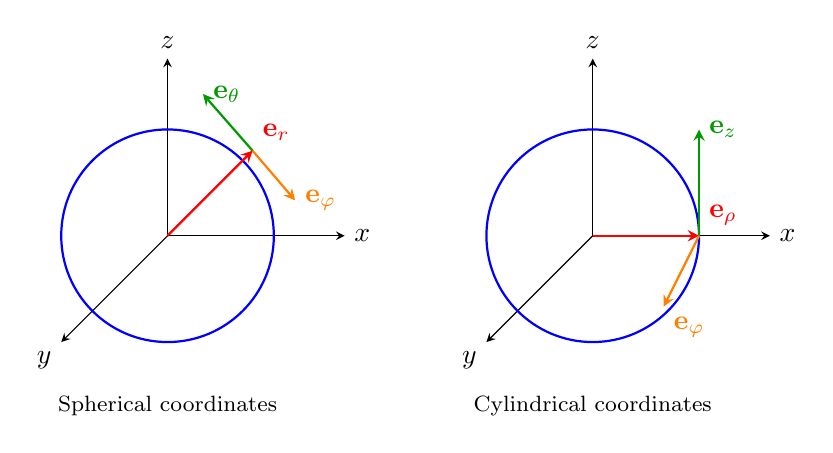
\begin{tikzpicture}[scale=0.9,>=stealth]
  % spherical coordinates
  \begin{scope}[shift={(0,0)}]
    \draw[->] (0,0) -- (2.5,0) node[right]{$x$};
    \draw[->] (0,0) -- (0,2.5) node[above]{$z$};
    \draw[->] (0,0) -- (-1.5,-1.5) node[below left]{$y$};
    \draw[thick, blue] (0,0) circle (1.5);
    \draw[->,thick,red] (0,0) -- (1.2,1.2) node[above right]{$\mathbf e_r$};
    \draw[->,thick,green!60!black] (1.2,1.2) -- (0.5,2.0) node[right]{$\mathbf e_\theta$};
    \draw[->,thick,orange] (1.2,1.2) -- (1.8,0.5) node[right]{$\mathbf e_\varphi$};
    \node[font=\footnotesize] at (0,-2.4) {Spherical coordinates};
  \end{scope}
  % cylindrical coordinates
  \begin{scope}[shift={(6,0)}]
    \draw[->] (0,0) -- (2.5,0) node[right]{$x$};
    \draw[->] (0,0) -- (0,2.5) node[above]{$z$};
    \draw[->] (0,0) -- (-1.5,-1.5) node[below left]{$y$};
    \draw[thick, blue] (0,0) circle (1.5);
    \draw[->,thick,red] (0,0) -- (1.5,0) node[above right]{$\mathbf e_\rho$};
    \draw[->,thick,green!60!black] (1.5,0) -- (1.5,1.5) node[right]{$\mathbf e_z$};
    \draw[->,thick,orange] (1.5,0) -- (1.0,-1.0) node[below right]{$\mathbf e_\varphi$};
    \node[font=\footnotesize] at (0,-2.4) {Cylindrical coordinates};
  \end{scope}
\end{tikzpicture}
\caption{Unit basis vectors in spherical and cylindrical coordinates.}
\label{fig:curvilinear_coordinates}
\end{figure}

\section{The inverse-square law}

\begin{remark}[The inverse-square law (statement in the chapter `Scalars and Vectors')]\label{thm:inverse_square_vector}
The conclusion of this section is exactly the same as \cref{thm:inverse_square} of the `Scalars and Vectors' chapter: if the flux of a central radial sourceless field through any closed surface enclosing the centre is the constant $\Phi_0$, then $F(r) = \Phi_0/(4\pi r^2)$. Both the statement and the proof are to be found there, and the discussion in the remainder of this section cites it directly.
\end{remark}

\begin{figure}[htbp]
    \centering
    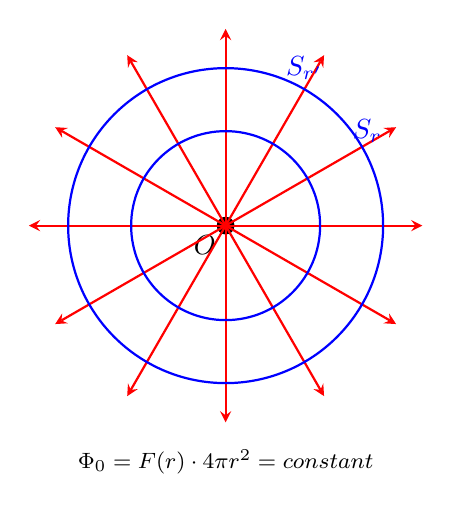
\begin{tikzpicture}[scale=1.0,>=stealth]
        \filldraw[black] (0,0) circle (3pt) node[below left] {$O$};
        \foreach \a in {0,30,...,330} {
            \draw[->, thick, red] (0,0) -- (\a:2.5);
        }
        \draw[blue, thick] (0,0) circle (1.2);
        \draw[blue, thick] (0,0) circle (2.0);
        \node[blue] at (1.8,1.2) {$S_r$};
        \node[blue] at (1.0,2.0) {$S_{r'}$};
        \node[font=\footnotesize] at (0,-3) {$\Phi_0 = F(r)\cdot 4\pi r^2 = \text{constant}$};
    \end{tikzpicture}
    \caption{Geometric derivation of the inverse-square law. The radial vector field passes through concentric spheres enclosing the source $O$, the total flux is conserved, and hence the field strength is inversely proportional to the square of the distance.}
    \label{fig:inverse_square}
\end{figure}

\begin{remark}[The converse and the conservation of flux (statement in the chapter `Scalars and Vectors')]\label{cor:inverse_square_converse_vector}
The same as \cref{cor:inverse_square_converse} of the `Scalars and Vectors' chapter: the flux of a radial field decaying like $C/r^2$ through any sphere centred at the centre is constantly $4\pi C$ (the field is sourceless for $r>0$, hence the same holds for any closed surface enclosing the centre); but `conservation of flux' and `inverse-square decay' are not unconditionally equivalent---they are two one-directional implications, whose exact scope is given in Remark \ref{rem:inverse_square_converse_scope} there. The proof is to be found there.
\end{remark}

\begin{remark}[Newton's law of universal gravitation and Coulomb's law (examples in the chapter `Scalars and Vectors')]
Taking the flux constant to be $\Phi_0 = -4\pi GM$ gives Newton's law of universal gravitation $\mathbf{g}(\mathbf{r}) = -G\frac{M}{r^2}\frac{\mathbf{r}}{r}$; taking $\Phi_0 = Q/\varepsilon_0$ gives Coulomb's law $\mathbf{E}(\mathbf{r}) = \frac{1}{4\pi\varepsilon_0}\frac{Q}{r^2}\frac{\mathbf{r}}{r}$. The complete derivations of the two examples are given in the `Scalars and Vectors' chapter (the two examples following \cref{thm:inverse_square}); here only the conclusions are listed and they are not repeated.
\end{remark}

\begin{example}[Counterexample: the inverse-square law fails if the flux is not constant]\label{ex:inverse_square_needs_const_flux}
The assumptions of \cref{thm:inverse_square_vector} include `the total flux of $\mathbf F$ through any closed surface enclosing $O$ is the constant $\Phi_0$'. Remove this clause and the conclusion fails.

Take $\mathbf F(\mathbf r) = f(r)\,\hat{\mathbf r}$, where $f(r) = 1/r^2$ for $r\in(0,1]$ and $f(r)=1/r^2+1$ for $r>1$. Then for $r>1$ the field is still spherically symmetric and sourceless outside $O$ ($\nabla\cdot\mathbf F=0$ holds on $\mathbb R^3\setminus\{O\}$ except on the sphere $r=1$), but the flux through a sphere of radius $r>1$ is
\[
\Phi(r) = 4\pi r^2\Bigl(\frac{1}{r^2}+1\Bigr) = 4\pi(1+r^2),
\]
which is not constant. Hence $F(r)$ does not have the form $\Phi_0/(4\pi r^2)$.

\textbf{Conclusion}: the clause `the flux is constant' in \cref{thm:inverse_square_vector} is not an automatic corollary of `sourceless + spherically symmetric' --- it is an \textbf{independent assumption}, whose physical meaning is `the total strength of the source is conserved'. In the present example extra sources appear on the sphere $r=1$ (as can be seen from $\nabla\cdot\mathbf F\ne0$), destroying the conservation of flux.
\end{example}

\section{Number of directions and angular resolution: from discrete to continuous}

\begin{definition}[Number of directions and angular resolution]\label{def:width_bandwidth}
For any period $T \in \mathbb{N}^+$:
\begin{enumerate}[label=(\roman*)]
    \item \textbf{Number of directions}: $N(T) = T$ --- the number of independent directions that the period $T$ is able to describe.
    \item \textbf{Angular resolution}: $\Delta\theta(T) = 2\pi/T$ --- the angular spacing between adjacent directions.
\end{enumerate}
The number of directions and the angular resolution satisfy the duality relation:
\[
N(T) \cdot \Delta\theta(T) = 2\pi.
\]
\end{definition}

\begin{figure}[htbp]
    \centering
    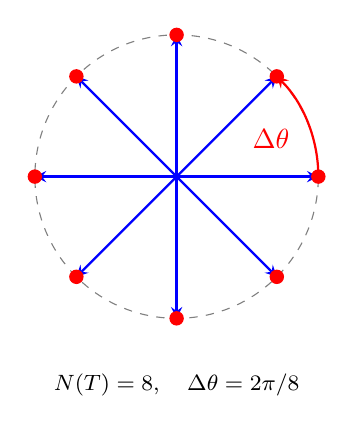
\begin{tikzpicture}[scale=1.2,>=stealth]
        \draw[gray, dashed] (0,0) circle (1.5);
        \foreach \k in {0,1,...,7} {
            \pgfmathsetmacro{\angle}{360*\k/8}
            \draw[->, thick, blue] (0,0) -- (\angle:1.5);
            \filldraw[red] (\angle:1.5) circle (2pt);
        }
        \draw[->, thick, red] (1.5,0) arc (0:45:1.5);
        \node[red] at (1.0,0.4) {$\Delta\theta$};
        \node[font=\footnotesize] at (0,-2.2) {$N(T)=8,\quad \Delta\theta=2\pi/8$};
    \end{tikzpicture}
    \caption{Number of directions and angular resolution. The period $T$ divides the circle into $T$ equal directions, and the angular spacing between adjacent directions is $\Delta\theta=2\pi/T$.}
    \label{fig:direction_resolution}
\end{figure}

\begin{definition}[Determining a coordinate point from the number of directions and the angular resolution]\label{def:coordinate_by_width_bandwidth}
Given a coordinate point $\mathbf{r} = (x, y) \neq \mathbf{0}$, let the argument be $\theta = \arctan2(y, x)$. The phase index is
\[
k(\mathbf{r}; T) = \left\lfloor \theta \cdot T / (2\pi) \right\rfloor \bmod T.
\]
The discrete representation is
\[
\mathbf{r}_T = \|\mathbf{r}\| \cdot e^{i2\pi k/T}.
\]
\end{definition}

\begin{theorem}[The limiting passage from discrete to continuous]\label{thm:discrete_to_continuous_limit}
Let $T_n \to \infty$. Then
\[
\lim_{n \to \infty} \mathbf{r}_{T_n} = \mathbf{r}.
\]
\end{theorem}

\begin{proof}
The discretisation error
\[
|\theta - 2\pi k/T_n| \le 2\pi/T_n \to 0.
\]
Therefore $\mathbf{r}_{T_n}\to \mathbf{r}$.
\end{proof}

\begin{definition}[Continuous number of directions and continuous angular resolution]\label{def:continuous_width_bandwidth}
In the continuous limit,
\[
N_{\infty} = \infty, \qquad \Delta\theta_{\infty} = 0,
\]
satisfying the limiting duality relation
\[
N_{\infty} \cdot \Delta\theta_{\infty} = 2\pi
\]
which holds in a generalised sense.
\end{definition}

\section{Periodic vector fields and the commutativity of the three differential operators}
\label{sec:periodic_vector_fields}

This chapter has used the gradient, divergence and curl together with the three integral theorems to characterise the behaviour of vector fields under the three basic transformations of translation, scaling and rotation. This section gives the entry point of the concept of `period' at the vector level: if a vector field is periodic in some translation direction, then the three differential operators preserve that periodicity; conversely, an operator preserving periodicity does not imply that the original field is periodic. This commutativity is the direct point of contact between this chapter and the `periodicity' theme of the whole book.

\begin{definition}[Periodic scalar fields and periodic vector fields]\label{def:periodic_vector_field}
Let $\mathbf a\in\mathbb R^3\setminus\{\mathbf 0\}$. A scalar field $f:\mathbb R^3\to\mathbb R$ is called \textbf{periodic} with respect to $\mathbf a$ if
\[
f(\mathbf x+\mathbf a)=f(\mathbf x),\qquad \forall \mathbf x\in\mathbb R^3 .
\]
A vector field $\mathbf F$ is called periodic with respect to $\mathbf a$ if all three of its components are so. The set of all $\mathbf a$ for which the above equation holds forms an additive subgroup of $\mathbb R^3$, denoted $\operatorname{Group}_{\mathrm{period}}(f)$ (or $\operatorname{Group}_{\mathrm{period}}(\mathbf F)$) and called the \textbf{group with periodic orbits} of the field.
\end{definition}

\begin{proposition}[The three differential operators commute with periodic translations]\label{prop:operators_commute_period}
Let $f$ be a $C^1$ scalar field and $\mathbf F$ a $C^1$ vector field, both periodic with respect to $\mathbf a$. Then
\begin{enumerate}[label=(\roman*)]
    \item Gradient: $(\nabla f)(\mathbf x+\mathbf a)=(\nabla f)(\mathbf x)$;
    \item Divergence: $(\nabla\cdot\mathbf F)(\mathbf x+\mathbf a)=(\nabla\cdot\mathbf F)(\mathbf x)$;
    \item Curl: $(\nabla\times\mathbf F)(\mathbf x+\mathbf a)=(\nabla\times\mathbf F)(\mathbf x)$.
\end{enumerate}
That is, all three differential operators \textbf{preserve invariance under periodic translations}.
\end{proposition}

\begin{proof}
(i) Let $\mathbf e$ be a unit vector. By the directional derivative and the chain rule,
\[
\mathbf e\cdot(\nabla f)(\mathbf x+\mathbf a)
=\frac{d}{dt}\Big|_{t=0}f(\mathbf x+\mathbf a+t\mathbf e)
=\frac{d}{dt}\Big|_{t=0}f(\mathbf x+t\mathbf e)
=\mathbf e\cdot(\nabla f)(\mathbf x),
\]
where the middle step uses $f(\mathbf y+\mathbf a)=f(\mathbf y)$ (taking $\mathbf y=\mathbf x+t\mathbf e$). Since $\mathbf e$ is arbitrary, (i) follows.

(ii)(iii) The divergence and the curl are both linear combinations of the gradient components (see \cref{def:divergence_vf} and \cref{def:curl_vf}); applying the corresponding sums and differences to (i) componentwise gives the conclusion.
\end{proof}

\begin{corollary}[The line integral along a periodic direction is zero]\label{cor:periodic_directional_integral_zero}
Let $f$ be a $C^1$ scalar field periodic with respect to $\mathbf a$. Then
\[
\int_0^{1}\mathbf a\cdot\nabla f(\mathbf x+t\mathbf a)\,dt=0 .
\]
That is: \textbf{the gradient of a periodic scalar field has no net increase along a periodic direction}.
\end{corollary}

\begin{proof}
By the chain rule, the integrand is exactly $\dfrac{d}{dt}f(\mathbf x+t\mathbf a)$, so the integral equals $f(\mathbf x+\mathbf a)-f(\mathbf x)=0$.
\end{proof}

\begin{remark}[Interface with the `periodicity' theme]\label{rem:vf_period_interface}
Proposition \ref{prop:operators_commute_period} and Corollary \ref{cor:periodic_directional_integral_zero} give the complete interface of this chapter with the `periodicity' theme:
\[
\begin{aligned}
&\text{translation symmetry (period)}\\
&\quad\Longrightarrow\ \text{the differential operators preserve that symmetry (conservation)}\\
&\quad\Longrightarrow\ \text{no net flux along a periodic direction (closure)}.
\end{aligned}
\]
This chain is used in the `Propagation and Evolution' chapter for Bloch--Floquet propagation in periodic media, and in the `Periodic Structure of Electromagnetic Systems' chapter for Maxwell's equations under periodic boundary conditions.
It must be noted that the \textbf{converse of (i) does not hold}: $\nabla f$ being periodic with respect to $\mathbf a$ does not imply that $f$ is periodic with respect to $\mathbf a$ --- for example, the gradient of $f(\mathbf x)=\mathbf e_1\cdot\mathbf x$ is a constant vector field (periodic with respect to every $\mathbf a$), whilst $f$ itself is not periodic. Hence the determination of periodicity must be carried out at the level of the original field, and one cannot look only at its derivative.
\end{remark}

\section*{Seven-theme comparison table for this chapter}

\begin{center}
\renewcommand{\arraystretch}{1.3}
\begin{tabular}{>{\centering\arraybackslash}p{2.2cm}>{\centering\arraybackslash}p{11cm}}
\toprule
Theme & Corresponding content in this chapter \\
\midrule
Translation & Gradient (symmetry centre $0$) $\nabla$ and directional derivatives; phase gradient of the time group \\
Scaling & Divergence (symmetry centre $1$) $\nabla\cdot$ and the inverse-square law \\
Rotation & Curl (symmetry centre $i$) $\nabla\times$ and circulation \\
Conservation & Gauss' theorem and Stokes' theorem; conservation laws of the space group \\
Symmetry & The correspondence between the differential operators and the three classes of basic symmetry generators, translation, scaling and rotation \\
Closure & Circulation and flux of closed curves/surfaces; the kernel of the projection operator \\
Period & The directional period given by the number of directions and the angular resolution \\
\bottomrule
\end{tabular}
\end{center}
\begin{table}[htbp]
    \centering
    \caption{Position and prerequisite dependencies of the structures of this chapter (for ease of checking and indexing)}
    \label{tab:chapter_structure_map}
    \renewcommand{\arraystretch}{1.2}
    \footnotesize
    \setlength{\tabcolsep}{4pt}
    \begin{tabular}{@{}l >{\raggedright\arraybackslash}p{3.1cm} >{\raggedright\arraybackslash}p{10.3cm}@{}}
        \toprule
        \textbf{Structure} & \textbf{Main location} & \textbf{Prerequisite dependency (what must be established first)} \\
        \midrule
        Definitions & sections \ref{sec:trans_scale_rotate} and \ref{sec:nabla_properties} and the sections that follow & none (definitions are the starting point of everything)\\
        Lemmas & $6$ in all, in sections \ref{sec:trans_scale_rotate} and \ref{sec:nabla_properties} & the corresponding definitions\\
        Propositions & $22$ in all, in sections \ref{sec:trans_scale_rotate} and \ref{sec:nabla_properties} and the sections that follow & the corresponding definitions and lemmas\\
        Theorems & $22$ in all, from section \ref{sec:trans_scale_rotate} onwards & the corresponding propositions and lemmas\\
        Proofs & immediately after each theorem and proposition & the object proved\\
        Corollaries & $11$ in all, from sections \ref{sec:nabla_properties} and \ref{sec:integral_theorems} onwards & the corresponding theorems\\
        Properties & $4$ in all, in the sections on the projection model and the sampling model & the corresponding definitions\\
        Examples & $26$ in all, with counterexamples distributed over the sections & the corresponding theorems and propositions\\
        Remarks & $17$ in all, used to delimit the scope of validity and the implicit assumptions & the corresponding conclusions\\
        \bottomrule
    \end{tabular}
\end{table}

\section*{Exercises}

\begin{enumerate}[leftmargin=3em, label=\textbf{Exercise \arabic*}]
    \item Prove Lemma \ref{lem:translation_group}: the translation group
    $(\mathcal{T}_n,\circ)$ forms an Abelian group, and
    \[
    (\mathcal{T}_n,\circ)\cong(\mathbb{R}^n,+).
    \]
    Please write out the complete verification of closure under composition, associativity, the identity element, the inverse element and the isomorphism.

    \item Prove Lemma \ref{lem:scaling_group}: the scaling group
    $(\mathcal{S}_n,\circ)$ forms an Abelian group, and
    \[
    (\mathcal{S}_n,\circ)\cong(\mathbb{R}_{>0},\times).
    \]
    Also explain why the scaling factor must satisfy $\lambda>0$ --- if $\lambda=0$ or
    $\lambda<0$ were allowed, what property would each of them break?

    \item Prove Proposition \ref{prop:similitude_group}:
    the group generated by translation, scaling and rotation is equal to the orientation-preserving similitude transformation group
    \[
    \mathrm{Sim}^{+}(n)=\{\mathbf{x}\mapsto\lambda R\mathbf{x}+\mathbf{a}\mid
    \lambda>0,\;R\in SO(n),\;\mathbf{a}\in\mathbb{R}^n\}.
    \]
    Please write out the proof of both directions of the inclusion relation, and explain why a reflection does not belong to this group.

    \item Verify Example \ref{ex:shear_anisotropic} that the shear transformation and anisotropic scaling do not belong to the similitude group:
    \[
    A_t=\begin{pmatrix}1&t\\0&1\end{pmatrix},\qquad
    B=\operatorname{diag}(2,1).
    \]
    Please compute $A_t^{\mathsf T}A_t$ and $B^{\mathsf T}B$ respectively,
    prove that neither of them is a scalar matrix, and hence that neither belongs to $\mathrm{Sim}^{+}(2)$.

    \item Prove Proposition \ref{prop:divergence_flux_density}:
    the divergence is the flux density,
    \[
    \nabla\cdot\mathbf{F}(\mathbf{x}_0)
    =\lim_{r\to0^+}\frac{1}{|B_r|}\oint_{\partial B_r}\mathbf{F}\cdot\mathbf{n}\,dS.
    \]
    Please complete the proof using the two fundamental integral identities on a sphere (Lemma \ref{lem:sphere_flux_identities})
    together with the first-order Taylor expansion.

    \item Prove Proposition \ref{prop:curl_circulation_density}:
    the curl is the circulation density,
    \[
    (\nabla\times\mathbf{F}(\mathbf{x}_0))\cdot\mathbf{n}
    =\lim_{r\to0^+}\frac{1}{|D_r|}\oint_{\gamma_r}\mathbf{F}\cdot d\mathbf{r}.
    \]
    Please take the disc $D_r$ through $\mathbf{x}_0$ with normal $\mathbf{n}$,
    expand $\mathbf{F}$ to first order and integrate term by term to complete the proof.

    \item Prove the three clauses of Theorem \ref{thm:infinitesimal_generators}:
    \begin{enumerate}[label=(\roman*)]
        \item the gradient and translation: $\frac{d}{dt}\big|_{t=0}f(\mathbf{x}+t\mathbf{a})=\mathbf{a}\cdot\nabla f(\mathbf{x})$;
        \item the divergence and the rate of change of volume: $\frac{d}{dt}\big|_{t=0}\operatorname{Vol}(\Phi_t(\Omega))=\int_\Omega\nabla\cdot\mathbf{F}\,dV$;
        \item the curl and the local angular velocity: $\frac12(J-J^{\mathsf T})\mathbf{y}=\frac12(\nabla\times\mathbf{F})\times\mathbf{y}$.
    \end{enumerate}
    Please complete the proof using the chain rule, the Jacobi formula and index computation respectively.

    \item Prove the six product rules in Theorem \ref{thm:product_rules}:
    \begin{enumerate}[label=(\roman*)]
        \item $\nabla(fg)=f\nabla g+g\nabla f$;
        \item $\nabla\cdot(f\mathbf{F})=f(\nabla\cdot\mathbf{F})+\nabla f\cdot\mathbf{F}$;
        \item $\nabla\times(f\mathbf{F})=f(\nabla\times\mathbf{F})+\nabla f\times\mathbf{F}$;
        \item $\nabla\cdot(\mathbf{F}\times\mathbf{G})=\mathbf{G}\cdot(\nabla\times\mathbf{F})-\mathbf{F}\cdot(\nabla\times\mathbf{G})$;
        \item the expansion of $\nabla\times(\mathbf{F}\times\mathbf{G})$;
        \item the expansion of $\nabla(\mathbf{F}\cdot\mathbf{G})$.
    \end{enumerate}
    Please complete all the proofs using the Levi-Civita symbol $\epsilon_{ijk}$ and the $\epsilon$-contraction identities.

    \item Prove Theorem \ref{thm:curl_grad_zero} and Theorem \ref{thm:div_curl_zero}:
    \[
    \nabla\times(\nabla f)=\mathbf{0},\qquad
    \nabla\cdot(\nabla\times\mathbf{F})=0.
    \]
    Please explain how the proofs of the two identities depend on Clairaut's mixed-partial-derivative interchange theorem (Lemma \ref{lem:clairaut}),
    and point out that the $C^2$ assumption cannot be omitted (see Counterexample \ref{ex:clairaut_failure}).

    \item Prove Theorem \ref{thm:laplacian_decomp}:
    \[
    \nabla^2\mathbf{F}=\nabla(\nabla\cdot\mathbf{F})-\nabla\times(\nabla\times\mathbf{F}).
    \]
    Please compute $(\nabla^2\mathbf{F})_1$ componentwise and verify that it equals the first component of the right-hand side,
    explaining that the two mixed-partial-derivative terms cancel by Clairaut's theorem.

    \item Prove Green's formula (Theorem \ref{thm:green_plane}):
    let $D$ be a bounded closed region with $\partial D$ piecewise smooth; then
    \[
    \iint_D\left(\frac{\partial Q}{\partial x}-\frac{\partial P}{\partial y}\right)dx\,dy
    =\oint_{\partial D}(P\,dx+Q\,dy).
    \]
    Please complete the proof in the three steps `prove it for a $y$-simple region, prove it for an $x$-simple region, sum over a general piecewise smooth boundary',
    and explain why the integrals over common edges of adjacent subregions cancel in pairs.

    \item Prove the curl theorem (Theorem \ref{thm:stokes}):
    \[
    \int_S(\nabla\times\mathbf{F})\cdot\mathbf{n}\,dS
    =\oint_{\partial S}\mathbf{F}\cdot d\mathbf{r}.
    \]
    Please complete the proof in the five steps `reduce to a graph surface $z=h(x,y)$, reduce to a double integral over $D$, apply Green's formula to $D$,
    restore the boundary integral, sum over a general piecewise smooth surface'.

    \item Prove the divergence theorem (Theorem \ref{thm:divergence}):
    \[
    \int_V(\nabla\cdot\mathbf{F})\,dV=\oint_{\partial V}\mathbf{F}\cdot\mathbf{n}\,dS.
    \]
    Please complete the proof in the three steps `the rectangular-box case, a $z$-simple region, a general regular region',
    and explain why the contributions of common faces of adjacent subregions cancel in pairs.

    \item Verify Counterexample \ref{ex:slit_domain_counterexample}:
    on the slit plane $\mathcal{M}=\mathbb{R}^2\setminus\{(x,0):x\ge0\}$,
    the vector field
    \[
    \mathbf{F}(x,y)=\left(\frac{-y}{x^2+y^2},\frac{x}{x^2+y^2}\right)
    \]
    satisfies $\nabla\times\mathbf{F}=\mathbf{0}$, but no scalar potential exists.
    Please compute the circulation along a closed curve winding once around the origin, and explain that the simple-connectivity condition cannot be omitted.

    \item Verify Counterexample \ref{ex:solenoidal_not_curl}:
    the vector field
    \[
    \mathbf{F}(\mathbf{x})=\frac{\mathbf{x}}{\|\mathbf{x}\|^3}
    \]
    satisfies $\nabla\cdot\mathbf{F}=0$ on $\mathbb{R}^3\setminus\{\mathbf{0}\}$,
    but is not the curl of any vector field.
    Please compute the flux through the unit sphere, and explain why zero divergence is not a sufficient condition.

    \item Prove the Helmholtz decomposition theorem (Theorem \ref{thm:helmholtz}):
    a suitably decaying vector field can be decomposed into the sum of an irrotational part and a solenoidal part:
    \[
    \mathbf{F}=-\nabla\phi+\nabla\times\mathbf{A}.
    \]
    Please explain that the existence of the decomposition depends on the Green's function of the Laplacian,
    and point out that uniqueness and the explicit integral formula require the decay condition (see Counterexample \ref{ex:helmholtz_decay_fails}).

    \item Verify Proposition \ref{prop:curvilinear_operators}:
    in the orthogonal curvilinear coordinate system $(\xi^1,\xi^2,\xi^3)$ with scale factors $h_i$,
    \begin{enumerate}[label=(\roman*)]
        \item $\nabla f=\sum_i\frac{1}{h_i}\frac{\partial f}{\partial\xi^i}\mathbf{e}_i$;
        \item $\nabla\cdot\mathbf{F}=\frac{1}{h_1h_2h_3}\sum_i
              \frac{\partial}{\partial\xi^i}\left(\frac{h_1h_2h_3}{h_i}F_i\right)$;
        \item $(\nabla\times\mathbf{F})_1=\frac{1}{h_2h_3}
              \left[\frac{\partial(h_3F_3)}{\partial\xi^2}
              -\frac{\partial(h_2F_2)}{\partial\xi^3}\right]$.
    \end{enumerate}
    Please write out the concrete expressions in spherical and cylindrical coordinates respectively (Example \ref{ex:spherical_cylindrical}).

    \item Prove the inverse-square law (Theorem \ref{thm:inverse_square}):
    if the total flux of a radial sourceless field through any closed surface enclosing the centre is the constant $\Phi_0$,
    then $F(r)=\Phi_0/(4\pi r^2)$.
    Please write out the flux computation, and prove its converse (Corollary \ref{cor:inverse_square_converse}).

    \item Verify Counterexample \ref{ex:inverse_square_needs_const_flux}:
    take $\mathbf{F}(\mathbf{r})=f(r)\hat{\mathbf{r}}$,
    where $f(r)=1/r^2$ ($r\le1$) and $f(r)=1/r^2+1$ ($r>1$).
    Please compute the flux through the sphere for $r>1$, verify that it is not constant,
    and explain that `the flux is constant' is an independent assumption and not an automatic corollary of sourcelessness plus spherical symmetry.

    \item Comprehensive question: combining the three basic transformations (Definitions \ref{def:translation_map}, \ref{def:scaling_map},
    \ref{def:rotation_map}), the three differential operators (Definitions \ref{def:gradient_vf},
    \ref{def:divergence_vf}, \ref{def:curl_vf})
    and the three integral theorems (Theorems \ref{thm:green_plane}, \ref{thm:stokes}, \ref{thm:divergence}),
    explain how vector analysis concretises, at the level of vector fields, the three great symmetry centres of periodic mathematics --- the additive symmetry centre $0$,
    the multiplicative symmetry centre $1$ and the rotational symmetry centre $i$.
    Please indicate which integral theorems correspond to conservation laws, and explain the difference in level among the three groups of objects
    (see Remark \ref{rem:centres_and_two_triples}).
\end{enumerate}
